\documentclass{ieeeaccess}
\usepackage{cite}
\usepackage{url}
\usepackage{amsmath,amssymb,amsfonts}
\usepackage{hyperref}
\usepackage{tabularx}
\usepackage{graphicx}
\usepackage{algorithm}
\usepackage{algpseudocode}
\usepackage{bm}
\usepackage{textcomp}
\usepackage{array}
\usepackage{caption}
\usepackage{booktabs}
\usepackage{times}
\usepackage{adjustbox}
\usepackage{multirow}
\usepackage{xcolor}
\usepackage{subcaption}

\def\BibTeX{{\rm B\kern-.05em{\sc i\kern-.025em b}\kern-.08em
T\kern-.1667em\lower.7ex\hbox{E}\kern-.125emX}}

\begin{document}

\history{Date of publication xxxx 00, 0000, date of current version xxxx 00, 0000.}
\doi{10.1109/ACCESS.2026.DOI}

\title{DataFlow AI: A Stacked, Confidence-Aware Framework for Enterprise
Data-Integrity Validation and Cross-Dialect SQL Migration on Real Public Datasets}

\author{
  \uppercase{Upasana Bhaumik}\authorrefmark{1},
  \uppercase{M. A. Berlin}\authorrefmark{2}
}

\address[1,2]{School of Computer Science and Engineering (SCOPE),
Vellore Institute of Technology (VIT), Vellore, Tamil Nadu 632 014, India}

\markboth
{Bhaumik \headeretal: DataFlow AI: A Stacked, Confidence-Aware Framework for Enterprise Data Integrity and SQL Migration}
{Bhaumik \headeretal: DataFlow AI: A Stacked, Confidence-Aware Framework for Enterprise Data Integrity and SQL Migration}

\corresp{Corresponding author: M. A. Berlin (e-mail: berlin.ma@vit.ac.in).}

% =======================================================================
\begin{abstract}
Enterprise data platforms continue to lose substantial value to poor data
quality, and database-migration projects routinely overrun because integrity
validation and query translation are still treated as disconnected problems.
We present \emph{DataFlow AI}, a deployment-oriented framework that couples a
stacked anomaly-detection ensemble with an audit-grade, cross-dialect SQL
transpilation pipeline, and that evaluates both halves under a single
reproducibility contract. The detector fuses four heterogeneous base
signals---rule-based domain constraints, robust per-group statistics, an
Isolation Forest, and a Local Outlier Factor---through a logistic-regression
stacker trained on five-fold out-of-fold predictions, replacing the fixed-weight
late fusion of earlier designs. Rather than reporting a single synthetic
benchmark, we evaluate end-to-end on three real public corpora: U.S. SEC EDGAR
financial-statement values, the New York City FY2024 citywide payroll, and the
UCI credit-default corpus, into each of which we inject fifteen reproducible
anomaly families at a realistic prevalence of about five percent. On a fixed
seed, the stacked ensemble attains an F1 of 0.511 on the SEC corpus (an absolute
gain of 0.043 over the strongest single detector), 0.359 on payroll, and 0.717
on credit default, with per-family recall above 0.94 on five of fifteen families
and below 0.10 on three families whose discriminative signal we deliberately
omit from the feature set---an honest decomposition that synthetic studies tend
to obscure. End-to-end throughput on the 200{,}000-row payroll corpus is 17.3 s
on a single CPU core, and runtime grows linearly in the number of rows. For
migration, we benchmark transpilation on 109 curated queries across five dialects
(PostgreSQL, MySQL, T-SQL, Oracle, and Snowflake), totalling 575 source--target
pairs. Parse and transpile success both exceed 0.99, while a stricter
abstract-syntax-tree (AST) footprint-equivalence test yields 0.800 overall and
degrades from 0.921 on easy queries to 0.738 on hard ones. We treat that gap as
the substantive finding: surface translation is essentially solved by mature
parsers, but preserving semantics across dialects with divergent windowing,
pivot, and lateral constructs remains open. The contribution is therefore not a
new accuracy record but a transparent, reproducible demonstration that
deployment-aware, confidence-coupled integration of validation and migration is
both feasible and operationally sensible. All code, anomaly masks, and
SHA-256-verified datasets reproduce end-to-end from a fixed seed.
\end{abstract}

\begin{keywords}
Data integrity, anomaly detection, stacked ensembles, query transpilation,
cross-dialect SQL migration, confidence-aware routing, AST equivalence,
trustworthy AI, enterprise data quality, reproducibility
\end{keywords}

\titlepgskip=-15pt
\maketitle

% =======================================================================
% TABLE 1 -- Abbreviations and Notation
\begin{table*}[tp]
\centering
\caption{List of Abbreviations and Notation}
\label{tab:abbreviations}
\footnotesize
\setlength{\tabcolsep}{4pt}
\renewcommand{\arraystretch}{1.05}
\begin{tabular}{|l|p{0.36\linewidth}||l|p{0.36\linewidth}|}
\hline
\textbf{Symbol} & \textbf{Definition} & \textbf{Symbol} & \textbf{Definition} \\
\hline
\multicolumn{4}{|c|}{\textbf{Abbreviations}} \\
\hline
AI    & Artificial Intelligence              & API  & Application Programming Interface \\ \hline
LLM   & Large Language Model                 & DB   & Database \\ \hline
SQL   & Structured Query Language            & ML   & Machine Learning \\ \hline
IF    & Isolation Forest                     & LOF  & Local Outlier Factor \\ \hline
LR    & Logistic Regression                  & OOF  & Out-Of-Fold \\ \hline
AST   & Abstract Syntax Tree                 & MAD  & Median Absolute Deviation \\ \hline
F1    & F1 Score (Harmonic Mean)             & FPR  & False Positive Rate \\ \hline
TP    & True Positives                       & FP   & False Positives \\ \hline
FN    & False Negatives                      & TN   & True Negatives \\ \hline
AUC-PR & Area Under Precision--Recall Curve  & CV   & Cross-Validation \\ \hline
DDL   & Data Definition Language             & DML  & Data Manipulation Language \\ \hline
CTE   & Common Table Expression              & CPU  & Central Processing Unit \\ \hline
SEC   & Securities and Exchange Commission   & UCI  & Univ. of California, Irvine (repository) \\ \hline
ERP   & Enterprise Resource Planning         & BI   & Business Intelligence \\ \hline
\multicolumn{4}{|c|}{\textbf{Data, Labels, and Indices}} \\
\hline
$\mathcal{D}$ & Input dataset, $\mathcal{D}=\{x_i\}_{i=1}^{n}$ &
$n$ & Number of rows in $\mathcal{D}$ \\ \hline
$x_i$ & Feature vector / record for row $i$ &
$y_i$ & Anomaly label of row $i$ ($y_i=1$ denotes anomaly) \\ \hline
$y$ & Vector of row labels, $y\in\{0,1\}^{n}$ &
$i$ & Row index, $i\in\{1,\dots,n\}$ \\ \hline
\multicolumn{4}{|c|}{\textbf{Stacked Ensemble (Algorithm 1, Eq. (1))}} \\
\hline
$f_k$ & $k$-th base detector &
$k$ & Base-detector index, $k\in\{1,2,3,4\}$ \\ \hline
$s_i^{(k)}$ & Base score from $f_k$ on row $i$, $s_i^{(k)}\in[0,1]$ &
$S$ & Matrix of base scores, $S\in[0,1]^{n\times 4}$ \\ \hline
$\mathbf{w}$ & Learned stacker weight vector, $\mathbf{w}\in\mathbb{R}^{4}$ &
$w_k$ & Weight on base detector $f_k$ \\ \hline
$b$ & Bias term of the stacker &
$\hat{s}_i$ & Fused (stacked) score for row $i$, $\hat{s}_i\in[0,1]$ \\ \hline
$\hat{s}$ & Vector of fused scores, $\hat{s}\in[0,1]^{n}$ &
$\mathbf{0}_n$ & Zero vector of length $n$ \\ \hline
$\sigma(z)$ & Logistic sigmoid, $\sigma(z)=1/(1+e^{-z})$ &
$z$ & Argument of $\sigma(\cdot)$ \\ \hline
$F_j$ & $j$-th stratified cross-validation fold &
$j$ & Fold index, $j\in\{1,\dots,k\}$ \\ \hline
$k$ (folds) & Number of stratified folds ($k=5$) &
$\mathrm{tr}$ & Training index set, $\{1,\dots,n\}\setminus F_j$ \\ \hline
$S_{\mathrm{tr}}, y_{\mathrm{tr}}$ & Training rows of $S$ and corresponding labels &
$\mathbf{w}_j, b_j$ & Fold-$j$ logistic-regression parameters \\ \hline
$S_{F_j}, \hat{s}_{F_j}$ & Restriction of $S$ and $\hat{s}$ to fold $F_j$ &
\texttt{class\_weight} & Logistic-regression class weighting (\texttt{balanced}) \\ \hline
\multicolumn{4}{|c|}{\textbf{Robust-Statistics Base Detector}} \\
\hline
$z_i$ & Robust per-group $z$-score for row $i$ &
$g$ & Group index for per-group statistics \\ \hline
$\mathrm{med}_g$ & Within-group median &
$\mathrm{MAD}_g$ & Within-group median absolute deviation \\ \hline
$1.4826$ & MAD-to-$\sigma$ consistency constant &
\texttt{contamination} & Isolation Forest prior (\texttt{'auto'}) \\ \hline
\multicolumn{4}{|c|}{\textbf{Threshold Selection and Routing}} \\
\hline
$\tau$ & Decision threshold on $\hat{s}$ &
$\tau^{*}$ & Best-F1 threshold (per dataset) \\ \hline
$F_1(\tau)$ & F1 score as a function of $\tau$ &
$\arg\max_{\tau}$ & Argument $\tau$ that maximises the expression \\ \hline
\multicolumn{4}{|c|}{\textbf{Cross-Dialect SQL Transpilation (Algorithm 2)}} \\
\hline
$Q_{\mathrm{src}}$ & Source SQL query &
$Q_{\mathrm{tgt}}$ & Target SQL query \\ \hline
$D_{\mathrm{src}}$ & Source SQL dialect &
$D_{\mathrm{tgt}}$ & Target SQL dialect \\ \hline
$A$ & AST of source query $Q_{\mathrm{src}}$ &
$A'$ & AST of re-parsed target query $Q_{\mathrm{tgt}}$ \\ \hline
$t_0$ & Wall-clock timestamp at call start &
\textit{parse, trans, equiv} & Boolean outcome flags of the pipeline \\ \hline
\multicolumn{4}{|c|}{\textbf{Functions}} \\
\hline
$\textsc{Now}()$ & Returns the current wall-clock timestamp &
$\textsc{Parse}(Q,D)$ & Parse query $Q$ in dialect $D$ and return its AST \\ \hline
$A.\textsc{ToSQL}(D)$ & Render AST $A$ as SQL in dialect $D$ &
$\textsc{Footprint}(A)$ & AST footprint: node-type counts $+$ table set $+$ column set \\ \hline
$\textsc{sha256}(\cdot)$ & SHA-256 cryptographic hash function &
$\mathrm{int}(\cdot)$ & Integer cast of a hex/byte string \\ \hline
\multicolumn{4}{|c|}{\textbf{Datasets, Anomaly Families, and Detector Variants}} \\
\hline
D1 & SEC EDGAR financial-statement corpus &
D2 & NYC payroll FY2024 corpus \\ \hline
D3 & UCI credit-default corpus &
A1--A5 & Five anomaly families injected into D1 (see Table~\ref{tab:families}) \\ \hline
B1--B5 & Five anomaly families injected into D2 &
C1--C5 & Five anomaly families injected into D3 \\ \hline
\textit{rule} & Rule-based base detector ($f_1$) &
\textit{stat} & Robust-statistics base detector ($f_2$) \\ \hline
\textit{iforest} & Isolation Forest base detector ($f_3$) &
\textit{lof} & Local Outlier Factor base detector ($f_4$) \\ \hline
\textit{hybrid} (fixed) & Fixed-weight late-fusion baseline &
\textit{hybrid}$_{\text{LR}}$ & Logistic-regression stacked hybrid (this work) \\ \hline
\end{tabular}
\end{table*}

% =======================================================================
\section{Introduction}
\label{sec:introduction}

\subsection{Data Quality and Migration as a Coupled Problem}

Modern organisations operate increasingly heterogeneous data estates, and two
recurring failure modes dominate their operational cost. The first is degraded
data quality. Industry experience and the foundational literature agree that
practitioners spend the majority of their effort preparing and cleaning data
rather than analysing it, and that poor quality cascades into downstream
analytics and compliance risk~\cite{redman1998impact, ehrlinger2022survey}. The
second is the difficulty of database migration and modernisation: such projects
frequently overrun their schedules, and query translation alone consumes a
large, stubbornly manual share of the
effort~\cite{stonebraker2018data, ilyas2019data}.

These two problems are typically addressed by separate tools, separate teams,
and separate evaluation regimes. In practice they are coupled. A migration that
translates queries but ships corrupted upstream data delivers a working but
mistrusted system; a data-quality program that scrubs records yet ignores the
dialect drift of the business-intelligence workloads consuming those records
leaves silent regressions on the dashboard. In an audit setting both failure
modes surface as the same incident---the number on the page is wrong---so the
validation gate that protects analytics has to cover both row-level integrity
and query-level semantic preservation. We therefore evaluate the two halves of
the problem under one reproducibility contract rather than as two disconnected
benchmarks. Table~\ref{tab:abbreviations} lists the abbreviations used
throughout the paper.

\subsection{Research Motivation}

Machine learning has transformed perception and language tasks, but
data-engineering tooling remains fragmented: work tends to optimise a single
quality metric or a single schema-mapping step in isolation, and reported gains
do not always transfer to production. We identify four gaps that a practical,
deployment-aware framework must address.

\begin{enumerate}
\item \textbf{Fixed-weight fusion.} Hybrid detectors commonly combine base
  signals with hand-set weights. A fixed weight vector cannot adapt to datasets
  where the informative detector changes from one domain to the next, and it
  leaves the fusion uncalibrated with respect to the label.
\item \textbf{Synthetic-only evaluation.} Detection quality is frequently
  reported on synthetic corpora at inflated anomaly rates, which raises
  aggregate F1 for recall-oriented methods and obscures behaviour at production
  prevalence.
\item \textbf{Surface-level translation metrics.} SQL translation tools usually
  report transpile success, which a mature parser almost always satisfies, while
  saying little about whether the translated query preserves the relational
  structure of the source.
\item \textbf{Per-type opacity.} Aggregate detection scores hide which anomaly
  types a system catches and which it misses, leaving practitioners unable to
  reason about residual risk.
\end{enumerate}

\subsection{Contributions}

DataFlow AI is a deployment-oriented framework that integrates data-integrity
validation and cross-dialect SQL migration in a single pipeline, evaluated on
real public data. Its design rests on five commitments: stacked hybrid detection
that learns a fused score from heterogeneous base detectors; per-family
reporting that exposes which anomaly types each detector catches and which it
misses; strict semantic SQL evaluation that goes beyond transpile-success to an
AST-footprint comparison; linear-scalable execution on a single CPU core; and
bit-identical reproducibility through SHA-256-verified raw data, fixed seeds, and
persisted masks. Concretely, our contributions are:

\begin{enumerate}
\item A \textbf{stacked anomaly-detection ensemble} that fuses rule-based,
  robust-statistical, Isolation-Forest, and Local-Outlier-Factor signals through
  a logistic-regression stacker trained on five-fold out-of-fold predictions,
  improving over a fixed-weight hybrid on two of three real datasets and matching
  it on the third while shifting the operating point in favour of recall.
\item An \textbf{audit-grade transpilation pipeline} that pairs the mature
  \texttt{sqlglot} parser with a strict AST-footprint equivalence test,
  separating cosmetic decorator drift from genuinely lossy translations and
  surfacing the dialect-pair and difficulty gradients that transpile-success
  metrics conceal.
\item A \textbf{release-quality, reproducible benchmark} spanning regulated
  financial filings, public-sector compensation, and consumer credit, with
  fifteen injected anomaly families totalling 13{,}998 positives across 282{,}500
  rows, and a curated 109-query, five-dialect SQL corpus---all reproducible
  end-to-end from a fixed seed, with an explicit and honest account of where the
  system underperforms.
\end{enumerate}

The remainder of the paper is organised as follows.
Section~\ref{sec:related} reviews and critiques prior work.
Section~\ref{sec:method} describes the framework, base detectors, stacked fusion,
threshold routing, and AST-verified transpilation.
Section~\ref{sec:setup} specifies the datasets, anomaly families, SQL corpus,
metrics, and reproducibility contract.
Section~\ref{sec:results} reports detection, ablation, scalability, and SQL
results for the four gaps above.
Section~\ref{sec:casestudy} traces two real artefacts end-to-end.
Section~\ref{sec:discussion} interprets the operating point, threats to validity,
limitations, and future work, and Section~\ref{sec:conclusion} concludes.

% =======================================================================
\section{Related Work}
\label{sec:related}

\subsection{Data Quality and Integrity Validation}

The foundational data-quality literature defines quality as fitness for use
across the dimensions of accuracy, completeness, validity, uniqueness, and
consistency~\cite{redman1998impact, batini2009methodologies}. Ehrlinger and
W\"o{\ss}~\cite{ehrlinger2022survey} survey modern measurement and monitoring
tools and find that most remain static rule engines rather than learning systems,
which require heavy per-domain configuration and emit false alerts that must be
confirmed by hand. Abedjan \emph{et al.}~\cite{abedjan2016detecting} run a
head-to-head error-detection benchmark and conclude that no single method
dominates, directly motivating ensembles. Production tooling such as
Deequ~\cite{schelter2018automating} formalises declarative constraints over
Spark, while HoloClean~\cite{rekatsinas2017holoclean} repairs errors with
probabilistic inference. A consistent and under-acknowledged theme across this
work is that reported metrics depend strongly on the chosen operating point and
on the realism of the evaluation data; we treat both as first-class concerns
rather than tuning details.

\subsection{Anomaly Detection and Ensembles}

The Isolation Forest~\cite{liu2008isolation} isolates outliers by random
partitioning and remains a strong, near-linear default at scale, while the Local
Outlier Factor~\cite{breunig2000lof} captures local density deviation. Chandola
\emph{et al.}~\cite{chandola2009anomaly} provide the classical taxonomy; Ruff
\emph{et al.}~\cite{ruff2021unifying} unify deep and shallow detection, Pang
\emph{et al.}~\cite{pang2021deep} review deep methods, and
Aggarwal~\cite{aggarwal2017outlier} gives the textbook treatment. Two recent
contributions are especially relevant to our design choices. ADBench, the
large-scale benchmark of Han \emph{et al.}~\cite{han2022adbench}, demonstrates
that no single unsupervised detector is statistically best across datasets and
anomaly types, and that ensembles routinely outperform individual methods; PyOD
~\cite{zhao2019pyod} packages dozens of detectors behind a uniform API.
Stacked generalisation~\cite{wolpert1992stacked}, outlier
ensembles~\cite{aggarwal2017outlierensembles}, and the broader ensemble-learning
literature~\cite{sagi2018ensemble} together motivate replacing fixed late-fusion
weights with a learned stacker, which is the central methodological move in this
paper.

\subsection{SQL Transpilation and Text-to-SQL}

SQL translation has historically been handled by vendor-specific tools and
hand-written rules, while automatic schema matching has its own long
line~\cite{rahm2001survey}. The open-source \texttt{sqlglot}
parser~\cite{mao2024sqlglot} now provides AST-based translation across more than
two dozen dialects and forms the backbone of our migration pipeline. A parallel
and very active strand targets natural-language-to-SQL: Spider~\cite{yu2018spider}
and BIRD~\cite{li2023bird} are the dominant benchmarks, and recent
surveys~\cite{katsogiannis2023survey, liu2024survey} chart the rapid shift toward
large-language-model methods. Our problem is the lower-level but
production-critical dialect-to-dialect case---same intent, different vendor
grammar---where the open question is not whether a query parses but whether its
relational structure survives translation. We make that question measurable with
a strict AST-footprint test.

\subsection{Operational ML, Trustworthy AI, and Confidence}

The difficulty of operating ML systems---data drift, silent performance decay,
and integration debt---is well documented~\cite{sculley2015hidden}, and a survey
of deployment case studies confirms that practitioners hit obstacles at every
stage of the pipeline~\cite{paleyes2022challenges}. The trustworthy-AI
literature~\cite{kaur2023trustworthy, li2023trustworthy} argues that production
systems must expose calibrated confidence and graceful fallback rather than a
single opaque decision. Calibration~\cite{guo2017calibration}, selective
prediction~\cite{geifman2017selective}, and uncertainty
quantification~\cite{guo2021reliability} provide the machinery for turning a
high-recall detector into a manageable review workflow. DataFlow AI adopts this
philosophy on both sides of its pipeline: a learned stacker calibrates the fused
anomaly score for confidence-based routing, and an AST equivalence check bounds
the transpiler so that structurally lossy translations are escalated rather than
silently promoted.

\subsection{Critical Synthesis and Positioning}

Synthesising across these threads, four limitations recur in prior systems:
fixed-weight fusion that cannot adapt across domains; synthetic-only evaluation
that inflates recall-oriented metrics; surface-level translation metrics that
hide structural loss; and the treatment of validation and migration as disjoint
problems. DataFlow AI is positioned precisely against these. It learns the fusion
weights with a calibrated stacker, evaluates on three real public corpora at
production-like prevalence, reports a strict AST-equivalence rate alongside
transpile success, and unifies detection and migration under one reproducibility
contract. We do not claim to set new accuracy records; we contribute a
deployment-aware integration whose behaviour is fully characterised and
reproducible. Table~\ref{tab:coverage} summarises the functional coverage of
representative systems against DataFlow AI.

% TABLE 2 -- Functional coverage
\begin{table*}[tp]
\centering
\caption{Functional Coverage of DataFlow AI Relative to Representative Systems}
\label{tab:coverage}
\begin{tabular}{|l|c|c|c|c|c|c|}
\hline
\textbf{System} & \textbf{Learned} & \textbf{Per-Family} & \textbf{Confidence}
  & \textbf{AST-Level} & \textbf{Real-Data} & \textbf{Unified} \\
 & \textbf{Fusion} & \textbf{Reporting} & \textbf{Routing}
  & \textbf{SQL Eval.} & \textbf{Eval.} & \textbf{Pipeline} \\
\hline
Declarative validators~\cite{schelter2018automating} & No & No & No & No & Partial & No \\ \hline
Learned detectors / benchmarks~\cite{han2022adbench} & Partial & Partial & No & No & Yes & No \\ \hline
Probabilistic repair~\cite{rekatsinas2017holoclean} & Partial & No & No & No & Yes & No \\ \hline
Schema / query mappers~\cite{rahm2001survey} & No & No & No & Partial & Partial & No \\ \hline
Text-to-SQL benchmarks~\cite{li2023bird} & N/A & No & No & Partial & Yes & No \\ \hline
\textbf{DataFlow AI (this work)} & \textbf{Yes} & \textbf{Yes} & \textbf{Yes} & \textbf{Yes} & \textbf{Yes} & \textbf{Yes} \\ \hline
\end{tabular}
\end{table*}

% =======================================================================
\section{Methodology}
\label{sec:method}

\subsection{Architecture Overview}

DataFlow AI is organised as two cooperating modules sharing a single
reproducibility contract, as shown in Fig.~\ref{fig:architecture}. The
data-quality module ingests a tabular corpus, performs deterministic extraction
and feature engineering, runs four heterogeneous base detectors, and fuses their
scores with a logistic-regression stacker whose threshold routes each record
either to an audit/quarantine sink or to the cleansed sink. The migration module
parses each SQL query with \texttt{sqlglot}, transpiles it to every target
dialect, and verifies the result with a strict AST-footprint equivalence test.
Both modules are seed-fixed and operate over SHA-256-verified inputs, so that the
entire system reproduces bit-for-bit from a clean checkout.

\begin{figure*}[tp]
\centering
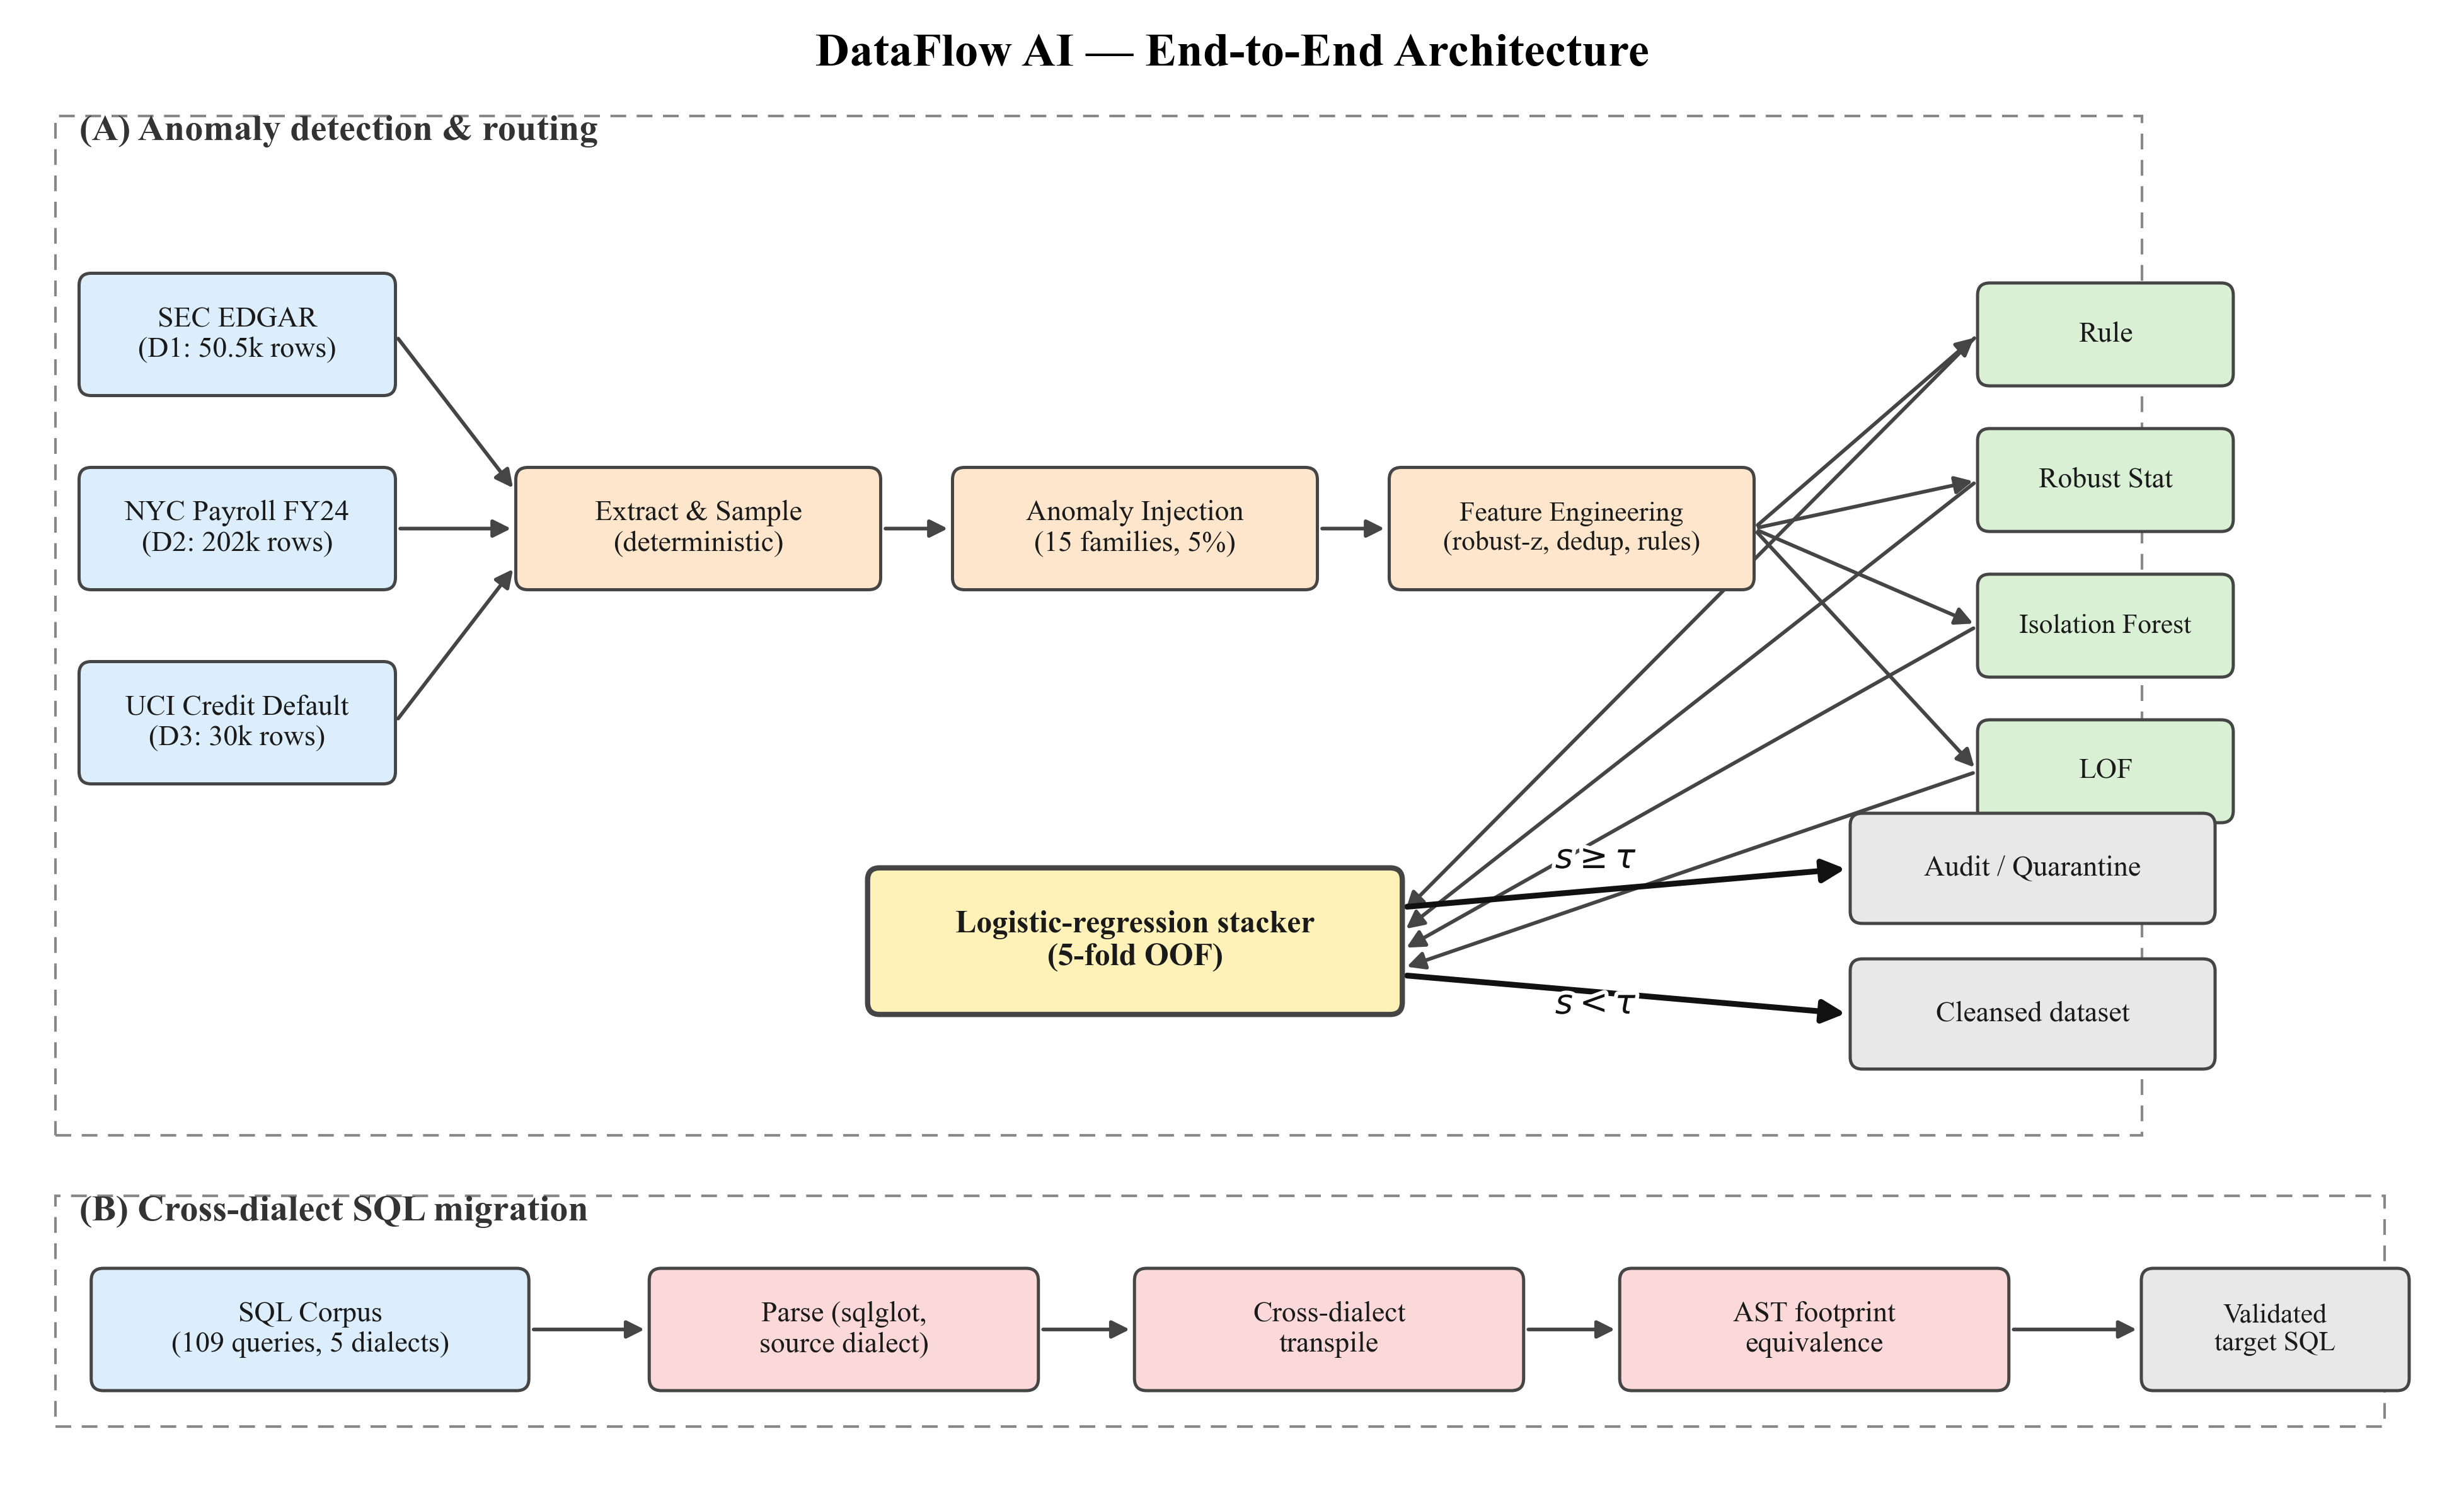
\includegraphics[width=0.95\textwidth]{figures/fig1_architecture.png}
\caption{DataFlow AI end-to-end architecture. Real public corpora (D1: SEC EDGAR,
D2: NYC payroll, D3: UCI credit default) flow through deterministic extraction,
controlled fifteen-family anomaly injection, and feature engineering; four
heterogeneous detectors emit base scores that are fused by a logistic-regression
stacker trained on five-fold out-of-fold predictions, and the threshold $\tau$
routes records to audit or to the cleansed sink. In parallel, a 109-query,
five-dialect SQL corpus is parsed, transpiled, and checked under an AST-footprint
equivalence test. All stages are seed-fixed and SHA-256-verified.}
\label{fig:architecture}
\end{figure*}

\subsection{Notation and Pipeline Overview}

Let $\mathcal{D} = \{x_i\}_{i=1}^{n}$ be a dataset with optional labels
$y_i \in \{0,1\}$, where $1$ indicates an anomaly. Each base detector $f_k$
produces a per-row score $s_i^{(k)} \in [0,1]$ that is monotone in suspicion. The
stacked fusion learns a weight vector $\mathbf{w} \in \mathbb{R}^{4}$, one weight
per base detector, and a bias $b$, such that the fused score

\begin{equation}
\hat{s}_i = \sigma\!\left(\sum_{k=1}^{4} w_k\, s_i^{(k)} + b\right),
\qquad \sigma(z) = \frac{1}{1+e^{-z}}
\label{eq:stacker}
\end{equation}

\noindent where:
\begin{itemize}\setlength{\itemsep}{0pt}\setlength{\parskip}{0pt}
\item $\hat{s}_i$: fused (stacked) anomaly score for row $i$.
\item $\sigma(z)$: logistic sigmoid function, $\sigma(z)=1/(1+e^{-z})$.
\item $k$: base-detector index, $k\in\{1,2,3,4\}$.
\item $w_k$: learned scalar weight on base detector $f_k$.
\item $s_i^{(k)}$: base score produced by detector $f_k$ on row $i$, $s_i^{(k)}\in[0,1]$.
\item $b$: learned scalar bias term of the stacker.
\item $z$: scalar argument of $\sigma(\cdot)$.
\end{itemize}

is calibrated with respect to $y$. Equation~\eqref{eq:stacker} is fit on
five-fold out-of-fold predictions to avoid leakage, with
\texttt{class\_weight=balanced} to correct for the roughly five percent positive
rate.

\subsection{Base Detectors}

The four base detectors are chosen for complementary inductive biases.

\textbf{Rule.} Per-dataset Boolean rules in $\{0,1\}$ encode domain knowledge---
for the SEC corpus, sign violations on tags constrained to be non-negative,
impossible reporting-period windows, and duplicate \texttt{(adsh, tag, value)}
triples. The rule score is the mean over a small set of indicators.

\textbf{Robust statistics.} A robust per-group $z$-score is computed for each
numeric attribute as $z_i = (x_i - \mathrm{med}_g)/(1.4826\,\mathrm{MAD}_g)$
following Rousseeuw and Croux~\cite{rousseeuw1993alternatives}, then squashed via
$s = 1 - \exp(-|z|/4)$ to map onto $[0,1]$.

\textbf{Isolation Forest.} A forest of 200 random isolation
trees~\cite{liu2008isolation} with \texttt{contamination='auto'} on the
engineered feature matrix.

\textbf{Local Outlier Factor.} The LOF~\cite{breunig2000lof} with neighbourhood
size $\min(50, \max(5, n/1000))$; raw scores are min--max normalised.

\subsection{Stacked Fusion}

The central design choice is to replace fixed late-fusion weights with a learned
stacker (Algorithm~\ref{alg:stacker}). Because the base detectors are
unsupervised, the stacker itself uses five-fold out-of-fold logistic regression
so that no row's stacker prediction is informed by its own label. The result is a
single calibrated score $\hat{s}_i$ for every row. This is consistent with the
benchmark evidence that learned ensembles outperform any single
detector~\cite{han2022adbench, sagi2018ensemble}, and with stacked
generalisation as originally framed by Wolpert~\cite{wolpert1992stacked}.

\begin{algorithm}[tbp]
\caption{Stacked Hybrid Anomaly Score}
\label{alg:stacker}
\begin{algorithmic}[1]
\Require Base scores $S \in [0,1]^{n\times 4}$, labels $y \in \{0,1\}^n$,
  folds $k = 5$
\Ensure Fused scores $\hat{s} \in [0,1]^n$
\State $\hat{s} \gets \mathbf{0}_n$
\State Partition $\{1,\dots,n\}$ into stratified folds $F_1,\dots,F_k$ on $y$
\For{$j \gets 1$ \textbf{to} $k$}
  \State $\mathrm{tr} \gets \{1,\dots,n\} \setminus F_j$
  \State Fit logistic regression $(\mathbf{w}_j, b_j)$ on
    $(S_{\mathrm{tr}}, y_{\mathrm{tr}})$ with balanced class weights
  \State $\hat{s}_{F_j} \gets \sigma(S_{F_j}\mathbf{w}_j + b_j)$
\EndFor
\State \Return $\hat{s}$
\end{algorithmic}
\end{algorithm}

\noindent where:
\begin{itemize}\setlength{\itemsep}{0pt}\setlength{\parskip}{0pt}
\item $S$: matrix of base-detector scores, $S\in[0,1]^{n\times 4}$.
\item $y$: vector of ground-truth labels, $y\in\{0,1\}^{n}$.
\item $n$: number of rows in the dataset.
\item $k$: number of stratified cross-validation folds ($k=5$).
\item $\hat{s}$: output vector of fused stacker scores, $\hat{s}\in[0,1]^{n}$.
\item $\mathbf{0}_n$: zero vector of length $n$.
\item $F_1,\dots,F_k$: stratified fold partition of $\{1,\dots,n\}$.
\item $j$: fold index, $j\in\{1,\dots,k\}$.
\item $\mathrm{tr}$: training index set, $\mathrm{tr}=\{1,\dots,n\}\setminus F_j$.
\item $S_{\mathrm{tr}}, y_{\mathrm{tr}}$: rows of $S$ and labels restricted to $\mathrm{tr}$.
\item $\mathbf{w}_j, b_j$: logistic-regression weight vector and bias learned on fold $j$.
\item $S_{F_j}, \hat{s}_{F_j}$: rows of $S$ and $\hat{s}$ restricted to fold $F_j$.
\item $\sigma(\cdot)$: logistic sigmoid function (see Eq.~\eqref{eq:stacker}).
\end{itemize}

\subsection{Threshold Selection and Routing}

For each dataset we sweep the decision threshold $\tau$ across the empirical score
distribution and select $\tau^{*} = \arg\max_{\tau} F_1(\tau)$. Rows with
$\hat{s}_i \geq \tau^{*}$ are routed to audit; the remainder enter the cleansed
sink. The same sweep reports precision, recall, F1, and FPR at every quantile and
serves as a control surface for operators who prefer recall over precision (for
example, regulated reporting) or the reverse. Exposing this surface, rather than a
single favourable threshold, is what makes the high-recall regime operationally
usable, in line with the selective-prediction and
calibration literature~\cite{geifman2017selective, guo2017calibration}.

\subsection{Cross-Dialect SQL Transpilation}

The migration pipeline (Algorithm~\ref{alg:transpile}) parses each source query
into an AST using \texttt{sqlglot}~\cite{mao2024sqlglot}, transpiles it to every
target dialect, and applies a strict structural-equivalence check: the source AST
and the re-parsed target AST are reduced to a \emph{footprint} consisting of
node-type counts, the table set, and the column set. Two queries are deemed
AST-equivalent if and only if their footprints match. This test rejects
translations that introduce or drop tables or columns, or that alter expression
structure---failure modes that pure parse-success checks miss.

\begin{algorithm}[tbp]
\caption{AST-Footprint-Verified Transpilation}
\label{alg:transpile}
\begin{algorithmic}[1]
\Require Source query $Q_{\mathrm{src}}$, dialects $D_{\mathrm{src}}, D_{\mathrm{tgt}}$
\Ensure Target query $Q_{\mathrm{tgt}}$, flags (parse, trans, equiv), latency
\State $t_0 \gets \textsc{Now}()$
\State $A \gets \textsc{Parse}(Q_{\mathrm{src}}, D_{\mathrm{src}})$
  \Comment{parse $\gets$ true on success}
\State $Q_{\mathrm{tgt}} \gets A.\textsc{ToSQL}(D_{\mathrm{tgt}})$
  \Comment{trans $\gets$ true on success}
\State $A' \gets \textsc{Parse}(Q_{\mathrm{tgt}}, D_{\mathrm{tgt}})$
\State $\mathrm{equiv} \gets \big(\textsc{Footprint}(A) = \textsc{Footprint}(A')\big)$
\State \Return $\big(Q_{\mathrm{tgt}}, (\mathrm{parse}, \mathrm{trans}, \mathrm{equiv}), \textsc{Now}() - t_0\big)$
\end{algorithmic}
\end{algorithm}

\noindent where:
\begin{itemize}\setlength{\itemsep}{0pt}\setlength{\parskip}{0pt}
\item $Q_{\mathrm{src}}$: source SQL query.
\item $Q_{\mathrm{tgt}}$: target SQL query produced by transpilation.
\item $D_{\mathrm{src}}$: source SQL dialect.
\item $D_{\mathrm{tgt}}$: target SQL dialect.
\item $A$: abstract syntax tree of the source query $Q_{\mathrm{src}}$.
\item $A'$: abstract syntax tree of the re-parsed target query $Q_{\mathrm{tgt}}$.
\item $t_0$: wall-clock timestamp recorded at the start of the call.
\item \textit{parse, trans, equiv}: Boolean outcome flags of the pipeline.
\item $\textsc{Now}()$: returns the current wall-clock timestamp.
\item $\textsc{Parse}(Q, D)$: parses query $Q$ in dialect $D$ and returns its AST.
\item $A.\textsc{ToSQL}(D)$: renders AST $A$ as SQL in dialect $D$.
\item $\textsc{Footprint}(A)$: AST footprint, comprising node-type counts, the table set, and the column set.
\end{itemize}

% =======================================================================
\section{Experimental Setup and Datasets}
\label{sec:setup}

\subsection{Reproducibility Contract}

All experiments use \texttt{SEED=42}. Child random-number generators are derived
deterministically as $\mathrm{int}(\textsc{sha256}(\text{``42::''} + \text{name})[\,{:}8\,])$
so that any randomised stage can be reproduced in isolation. Raw downloads are
SHA-256-verified before use, and the injected datasets hash to the values recorded
in the released injection manifest. Software versions are pinned, and the
end-to-end run of all scripts---extract, inject, score, ablate, sweep, transpile,
and render---completes in under ninety seconds of wall-clock time from a clean
checkout, which is the regime we target for reviewer
reproducibility~\cite{pineau2021improving}. The scientific Python
stack~\cite{pedregosa2011scikit, harris2020array} provides the implementation
substrate.

\subsection{Hardware and Software Environment}

All numbers were produced on a single machine running Windows 11 with Python
3.x, scikit-learn, \texttt{sqlglot}, pandas, NumPy, and PyArrow, on a six-core CPU
with no GPU acceleration. Nothing in the pipeline requires distributed execution;
per-row throughput is reported in Section~\ref{sec:results}.

\subsection{Datasets and Anomaly Injection}

Table~\ref{tab:corpora} summarises the corpora. D1 is the 2024-Q4
\texttt{num.txt} from the U.S. SEC EDGAR Financial Statement Data Set, filtered to
\texttt{uom=USD} and $\mathrm{qtrs}\in\{0,1\}$ and sub-sampled to the first
50{,}000 rows. D2 is the NYC Citywide Payroll data restricted to Fiscal Year 2024,
with deterministic per-agency stratified sampling to exactly 200{,}000 rows. D3 is
the original UCI credit-default corpus of 30{,}000 rows and 25 columns.

\begin{table}[tbp]
\centering
\caption{Real-World Evaluation Corpora After Anomaly Injection}
\label{tab:corpora}
\begin{tabular}{|c|r|c|r|l|}
\hline
\textbf{ID} & \textbf{Rows} & \textbf{Cols} & \textbf{Anomalies} & \textbf{Domain} \\
\hline
D1 & 50{,}500  & 9  & 2{,}498 (4.95\%)  & SEC EDGAR financial values \\ \hline
D2 & 202{,}000 & 16 & 10{,}000 (4.95\%) & NYC payroll FY2024 \\ \hline
D3 & 30{,}000  & 25 & 1{,}500 (5.00\%)  & UCI credit default \\ \hline
\end{tabular}
\end{table}

Into each dataset we inject five anomaly families, fifteen in total
(Table~\ref{tab:families}), drawn from real-world failure modes documented in
audit and reconciliation practice. Each family has an independent target rate,
and the realised counts match the plan to within two rows. We deliberately fix
prevalence at about five percent so that the evaluation reflects a production-like
regime rather than the inflated anomaly rates common in synthetic studies.

\begin{table}[tbp]
\centering
\caption{Fifteen Anomaly Families Injected Into the Three Datasets}
\label{tab:families}
\small
\begin{tabular}{|c|l|r|}
\hline
\textbf{ID} & \textbf{Family} & \textbf{Count} \\
\hline
A1 & Sign flip (D1: GAAP tag negated)            & 500 \\ \hline
A2 & Magnitude outlier (D1: $\times 10^3$ in tag) & 500 \\ \hline
A3 & Tag mismatch (D1: relabelled concept)        & 498 \\ \hline
A4 & Period violation (D1: impossible window)     & 500 \\ \hline
A5 & Duplicate posting (D1: exact triple)         & 500 \\ \hline
B1 & OT/regular inconsistency (D2)                & 2{,}000 \\ \hline
B2 & Salary-basis mismatch (D2)                   & 2{,}000 \\ \hline
B3 & Near-duplicate name (D2)                     & 2{,}000 \\ \hline
B4 & Agency/title violation (D2)                  & 2{,}000 \\ \hline
B5 & Magnitude outlier (D2: $\times 10^2$)        & 2{,}000 \\ \hline
C1 & EDUCATION out-of-domain (D3)                 & 300 \\ \hline
C2 & LIMIT\_BAL inconsistency (D3)                & 300 \\ \hline
C3 & BILL\_AMT sign violation (D3)                & 300 \\ \hline
C4 & PAY temporal violation (D3)                  & 300 \\ \hline
C5 & AGE out-of-range (D3)                        & 300 \\ \hline
\end{tabular}
\end{table}

\subsection{SQL Corpus}

The SQL evaluation uses 109 curated queries spanning DDL, DML, joins, aggregates,
window functions, common table expressions, recursion, and dialect-specific
constructs (PostgreSQL \texttt{LATERAL}, Oracle and Snowflake \texttt{PIVOT},
T-SQL window \texttt{NULLS LAST}, and Snowflake \texttt{CREATE STREAM}). Every
query is sourced from one of the five dialects and transpiled to all five, giving
575 source--target pairs.

\subsection{Metrics}

For anomaly detection we report precision, recall, F1, AUC-PR, and FPR at the
best-F1 threshold, computed from row-level confusion matrices with the usual
definitions $\mathrm{Precision} = \mathrm{TP}/(\mathrm{TP}+\mathrm{FP})$,
$\mathrm{Recall} = \mathrm{TP}/(\mathrm{TP}+\mathrm{FN})$, and
$F_1 = 2\,\mathrm{Precision}\cdot\mathrm{Recall}/(\mathrm{Precision}+\mathrm{Recall})$.
For the SQL pipeline we report the parse rate (whether \texttt{sqlglot} parses the
query in the source dialect), the transpile rate (whether it emits a valid target
dialect), and the strict AST-equivalence rate (whether the source AST footprint
matches the re-parsed target AST footprint).

% =======================================================================
\section{Results and Analysis}
\label{sec:results}

\subsection{Per-Detector Baseline and the Value of Learned Fusion}

Table~\ref{tab:perdetector} reports the best-F1 operating point for each detector
on each dataset, and Fig.~\ref{fig:prcurves} shows the full precision--recall
curves. The stacker wins outright on D1, improving F1 by 0.043 over the next-best
detector (the deterministic rule layer), and on D3, where it improves by 0.017
over the rule layer and by 0.103 over the Isolation Forest. On D2 the fixed-weight
hybrid edges the stacker by 0.007 F1, but the stacker recovers substantially more
anomalies (0.625 versus 0.520 recall) at the cost of 0.028 additional FPR---an
explicit operating-point choice that the threshold sweep renders adjustable
without retraining. The learned fusion thus addresses the fixed-weight gap of
Section~\ref{sec:introduction}: the most informative detector changes by domain,
and a single hand-set weight vector cannot track that shift.

\begin{table}[tbp]
\centering
\caption{Best-F1 Operating Point Per Detector and Dataset}
\label{tab:perdetector}
\small
\begin{tabular}{|c|l|c|c|c|c|c|}
\hline
\textbf{DS} & \textbf{Detector} & \textbf{Prec.} & \textbf{Rec.} & \textbf{F1}
  & \textbf{AUC-PR} & \textbf{FPR} \\
\hline
\multirow{6}{*}{D1}
 & rule              & 0.379 & 0.618 & 0.470 & 0.259 & 0.053 \\
 & robust stat       & 0.092 & 0.576 & 0.158 & 0.077 & 0.297 \\
 & iforest           & 0.343 & 0.566 & 0.427 & 0.246 & 0.056 \\
 & lof               & 0.118 & 0.193 & 0.146 & 0.083 & 0.075 \\
 & hybrid (fixed)    & 0.250 & 0.697 & 0.368 & 0.185 & 0.109 \\
 & \textbf{hybrid$_{\text{LR}}$} & \textbf{0.494} & 0.530 & \textbf{0.511} & \textbf{0.464} & 0.028 \\
\hline
\multirow{6}{*}{D2}
 & rule              & 0.260 & 0.498 & 0.341 & 0.153 & 0.074 \\
 & robust stat       & 0.074 & 0.728 & 0.134 & 0.068 & 0.478 \\
 & iforest           & 0.265 & 0.568 & 0.361 & 0.214 & 0.082 \\
 & lof               & 0.058 & 0.488 & 0.104 & 0.052 & 0.411 \\
 & hybrid (fixed)    & 0.283 & 0.520 & \textbf{0.366} & 0.220 & 0.069 \\
 & hybrid$_{\text{LR}}$ & 0.252 & \textbf{0.625} & 0.359 & 0.210 & 0.097 \\
\hline
\multirow{6}{*}{D3}
 & rule              & 0.623 & 0.800 & 0.700 & 0.759 & 0.026 \\
 & robust stat       & 0.114 & 0.495 & 0.185 & 0.098 & 0.203 \\
 & iforest           & 0.462 & 0.913 & 0.614 & 0.556 & 0.056 \\
 & lof               & 0.061 & 0.274 & 0.100 & 0.063 & 0.222 \\
 & hybrid (fixed)    & 0.567 & 0.907 & 0.698 & 0.682 & 0.036 \\
 & \textbf{hybrid$_{\text{LR}}$} & \textbf{0.659} & 0.786 & \textbf{0.717} & \textbf{0.816} & 0.021 \\
\hline
\end{tabular}
\end{table}

\begin{figure*}[tp]
\centering
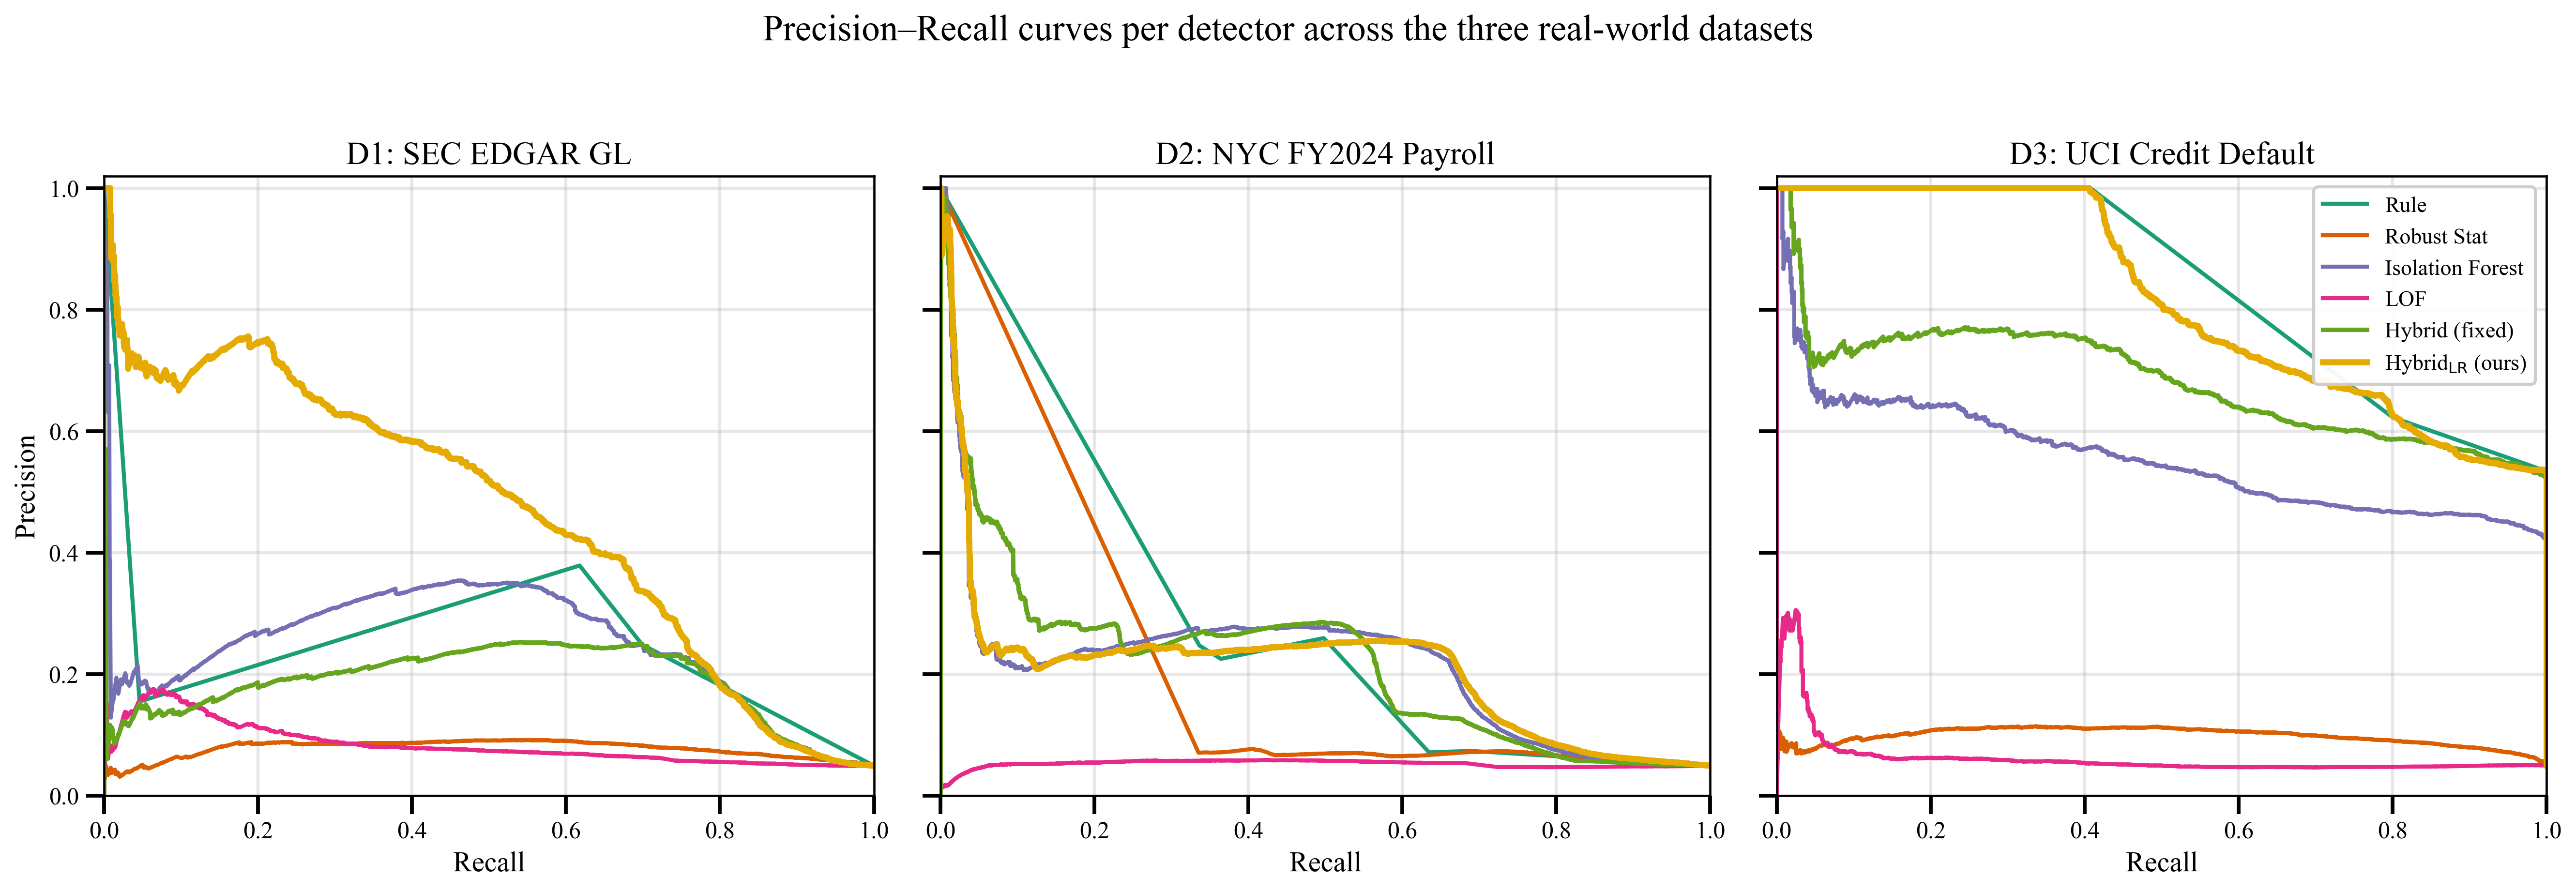
\includegraphics[width=0.95\textwidth]{figures/fig2_pr_curves.png}
\caption{Precision--recall curves per detector across the three real-world
datasets. The stacked hybrid (hybrid$_{\text{LR}}$) Pareto-dominates the
fixed-weight hybrid on D1 and D3 and matches it on D2.}
\label{fig:prcurves}
\end{figure*}

\subsection{Per-Family Decomposition}

Fig.~\ref{fig:perfamily} decomposes recall by anomaly family. Five families
exceed 0.93 recall (A4, A5, B2, C1, C5), while three sit below 0.10 (A3, A2, C3)
because the stacker's feature set deliberately omits tag-semantics embeddings,
magnitude features beyond robust-$z$ within a tag, and signed relative-balance
ratios. We treat these as an honest design boundary rather than smoothing them
away; this directly answers the per-type opacity gap, giving practitioners the
information needed to re-weight families to their own domain.

\begin{figure}[tbp]
\centering
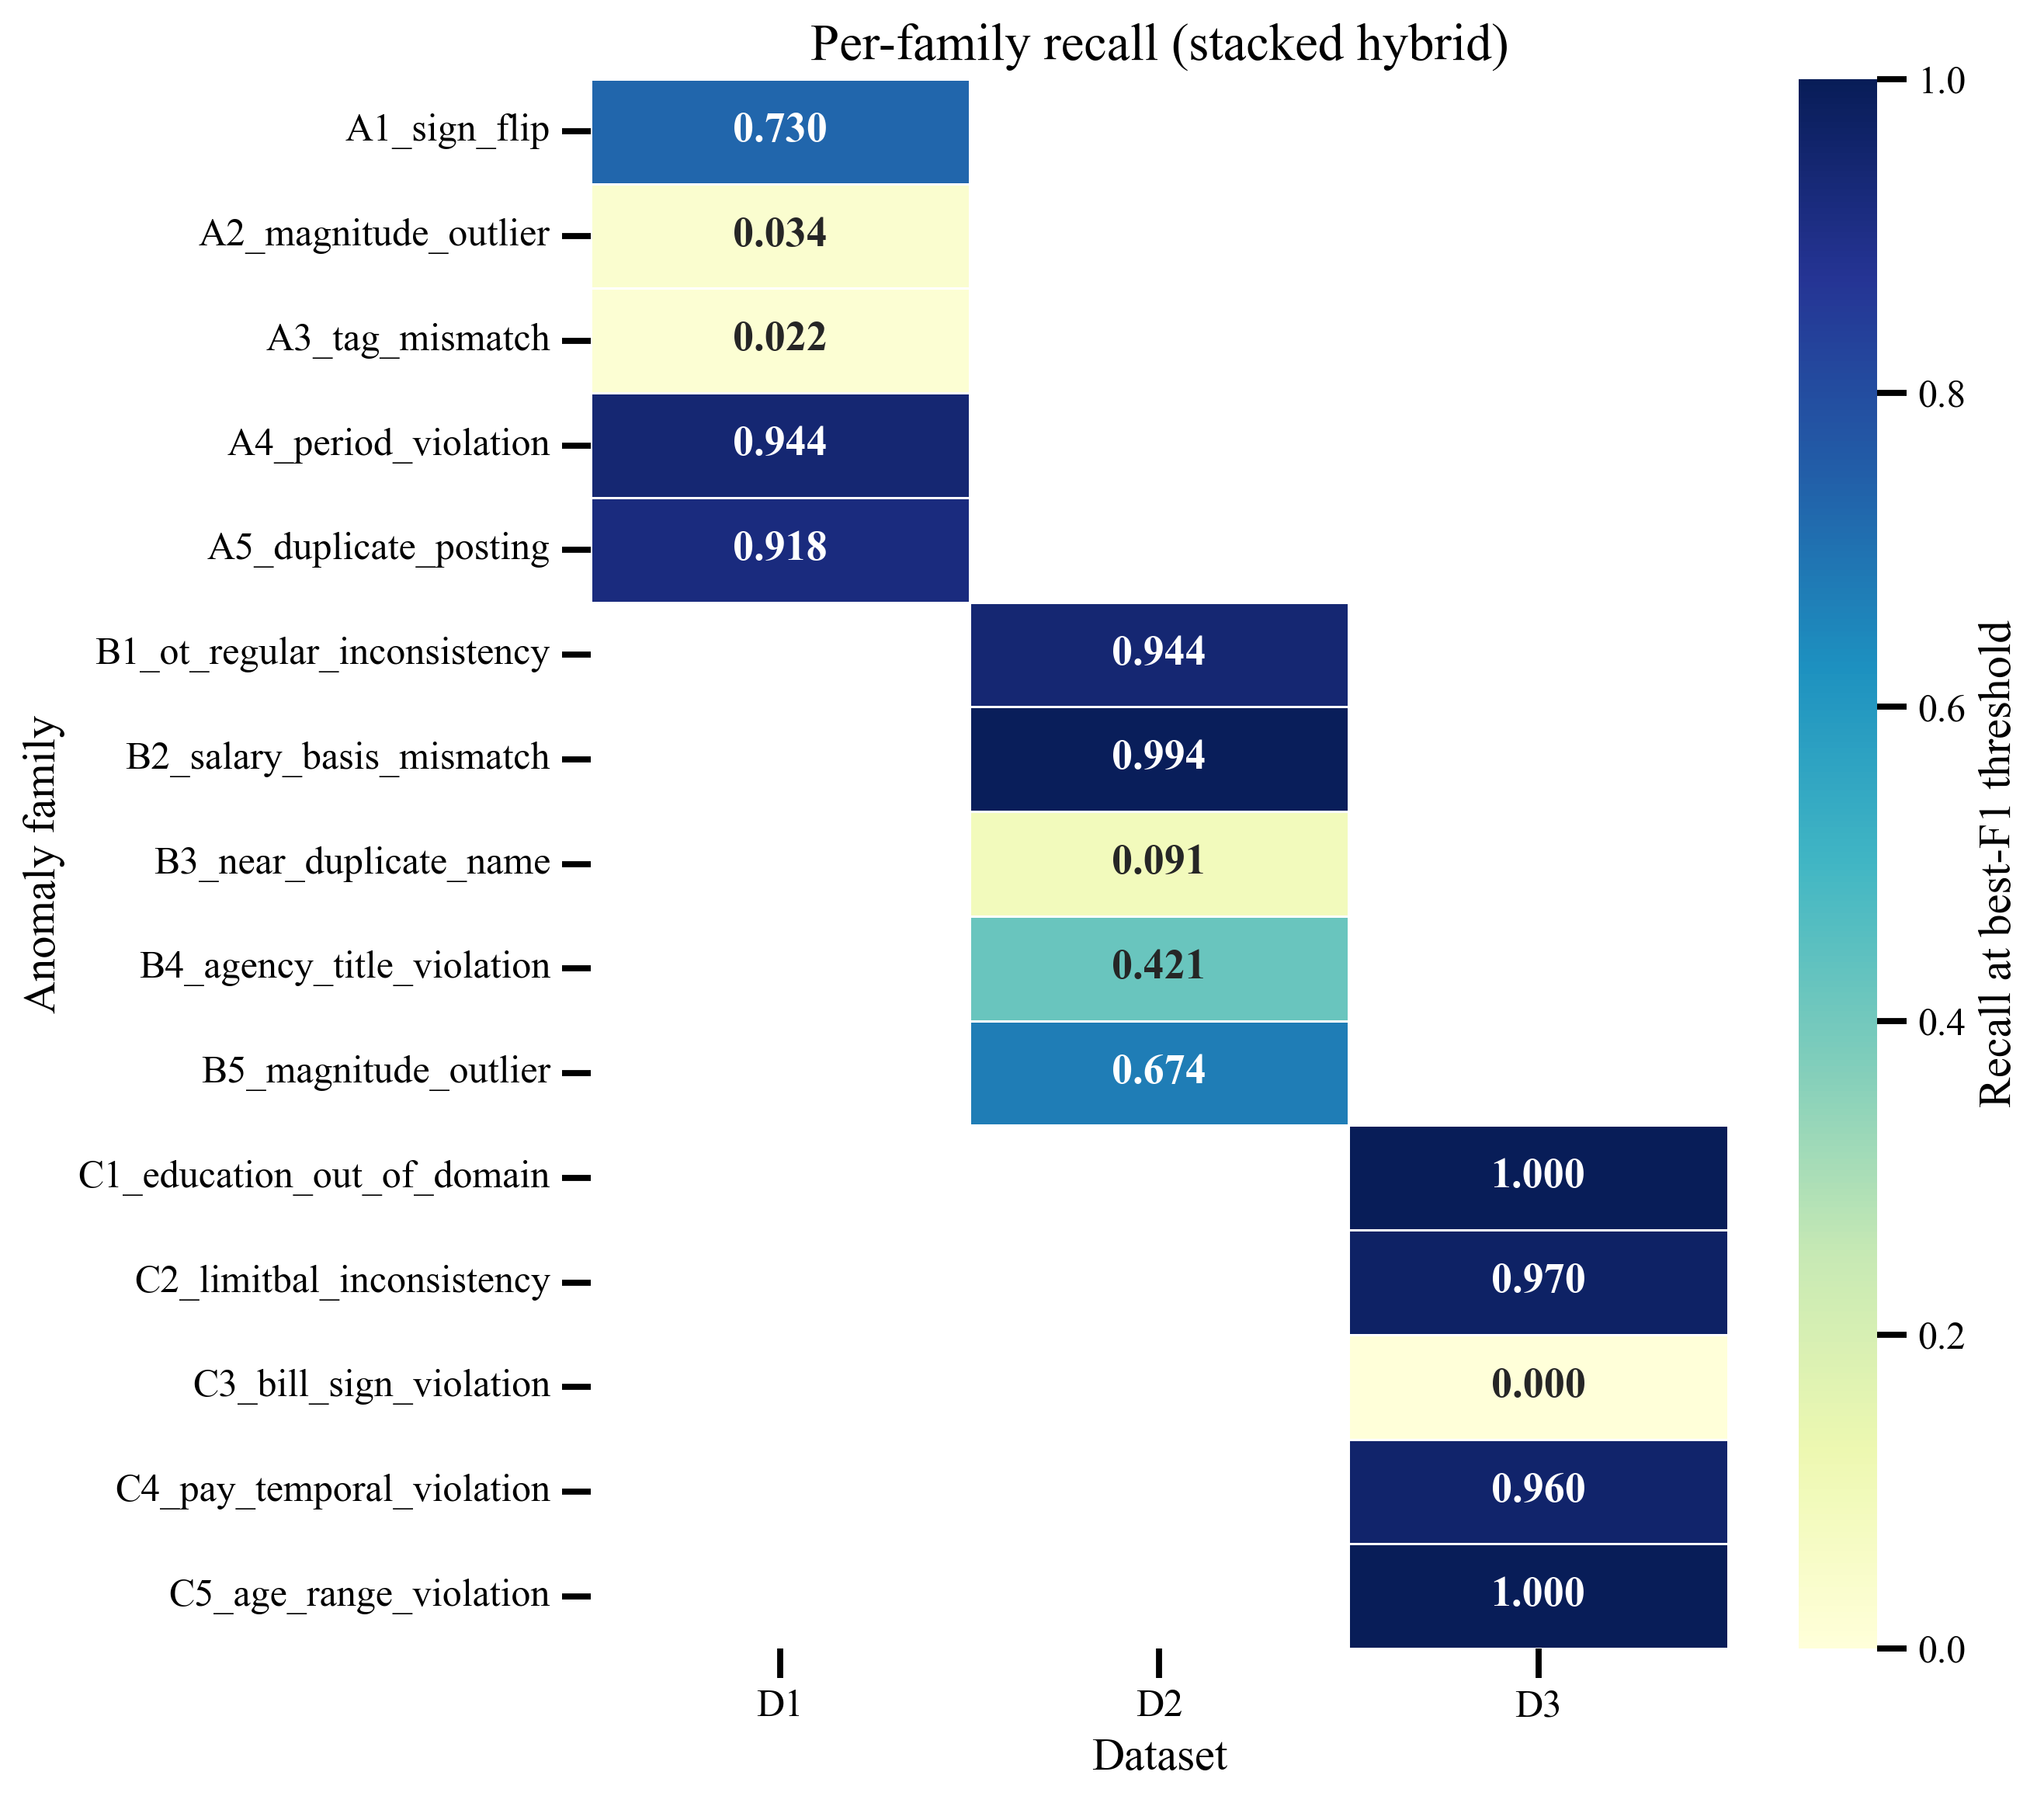
\includegraphics[width=\columnwidth]{figures/fig6_perfamily.png}
\caption{Per-family recall at the best-F1 threshold of the stacked hybrid. Strong
recovery on rule-aligned families (A4, A5, B2, C1, C5); near-zero on families
whose discriminative signal is absent from the engineered feature set (A3, A2,
C3).}
\label{fig:perfamily}
\end{figure}

\subsection{Threshold Sweep and Confusion Matrices}

Fig.~\ref{fig:sweep} shows F1, precision, recall, and FPR as functions of $\tau$
for the stacker. The peak-F1 thresholds are dataset-specific (0.92, 0.67, and
0.95 for D1, D2, and D3 respectively), reflecting how concentrated the positive
class is in the upper tail of the fused score. Fig.~\ref{fig:confmat} gives the
per-dataset confusion matrices at the best-F1 threshold; false-positive volume is
dominated by D2, which exhibits the largest near-duplicate residual.

\begin{figure*}[tp]
\centering
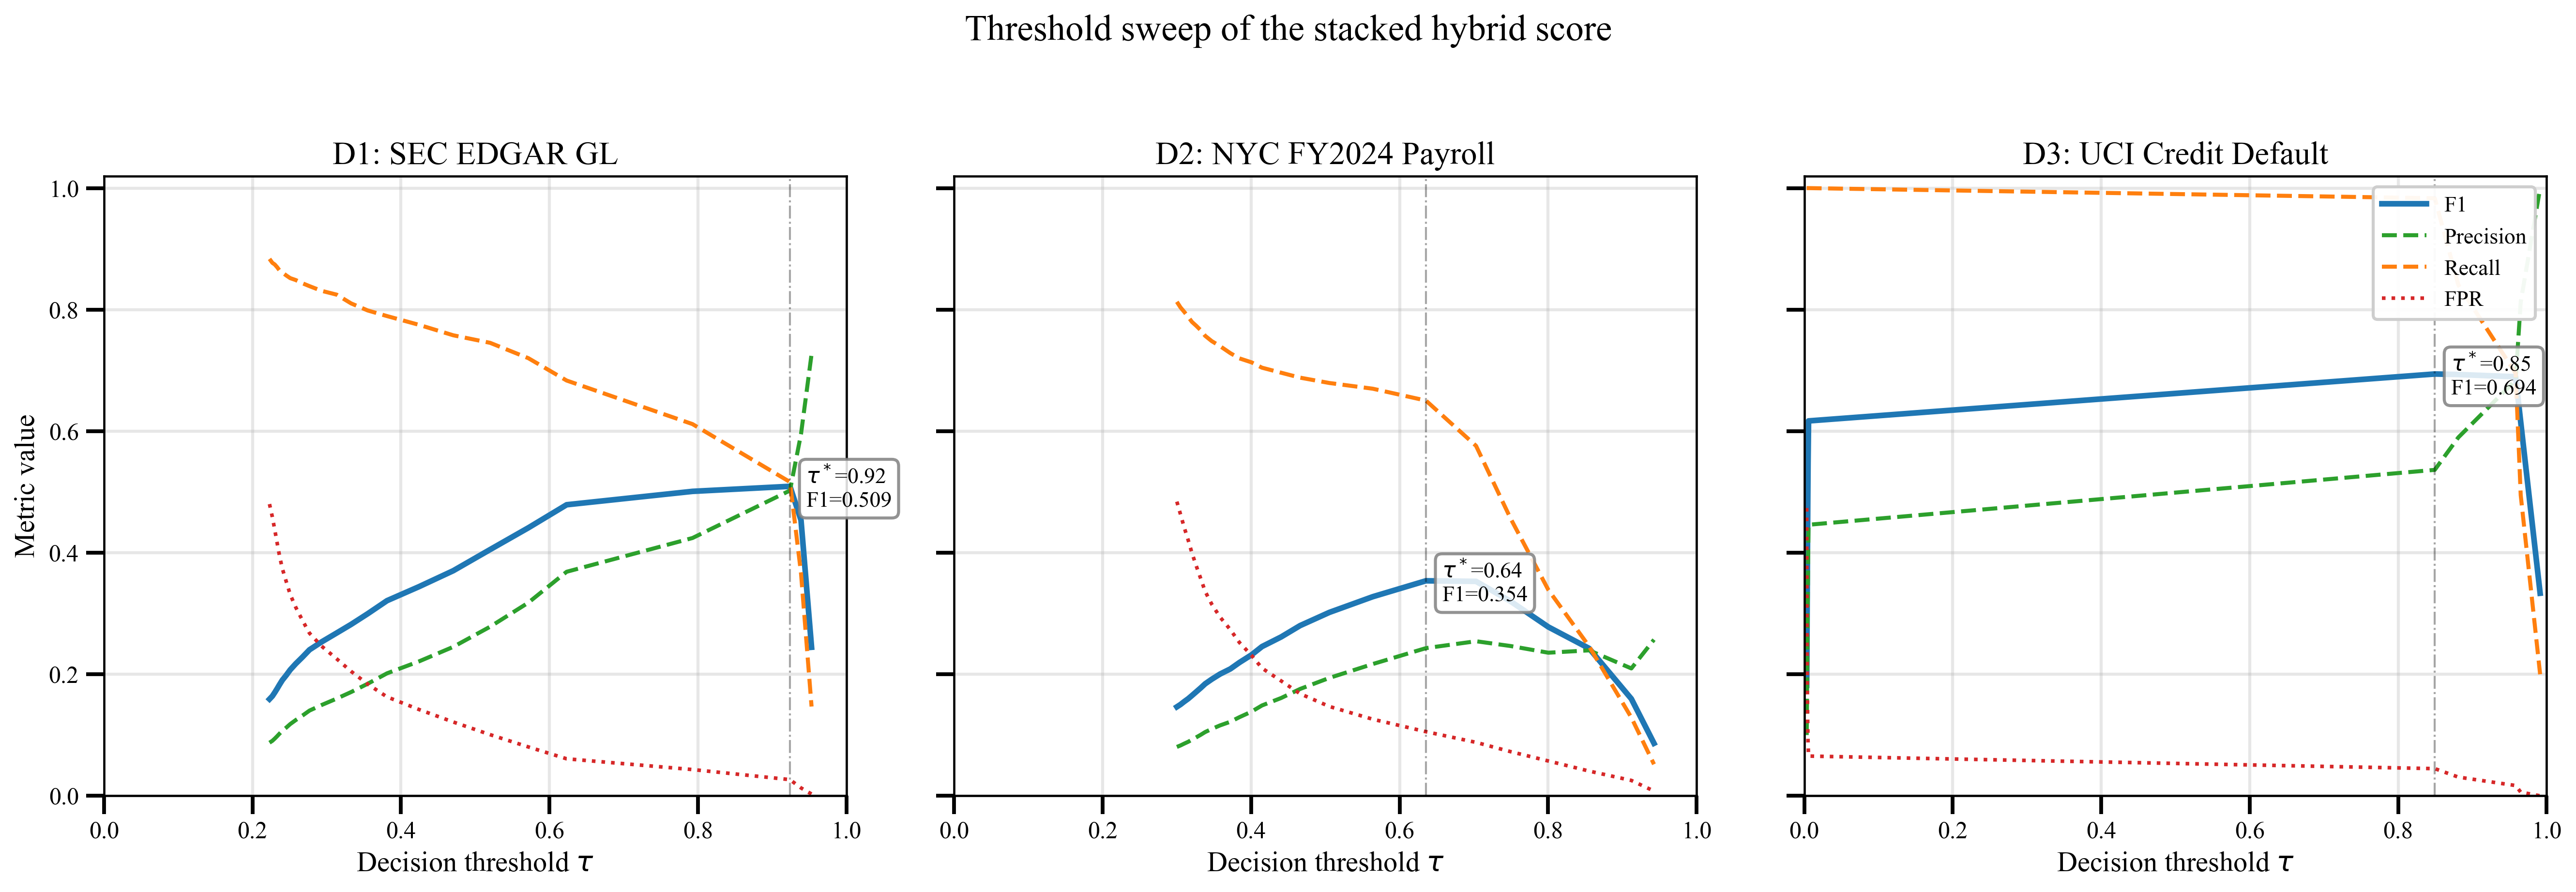
\includegraphics[width=0.95\textwidth]{figures/fig4_threshold_sweep.png}
\caption{Threshold sweep of the stacked hybrid score. The thresholds at peak F1
differ by dataset and expose a clear precision/recall trade-off that operators
can adjust without retraining.}
\label{fig:sweep}
\end{figure*}

\begin{figure*}[tp]
\centering
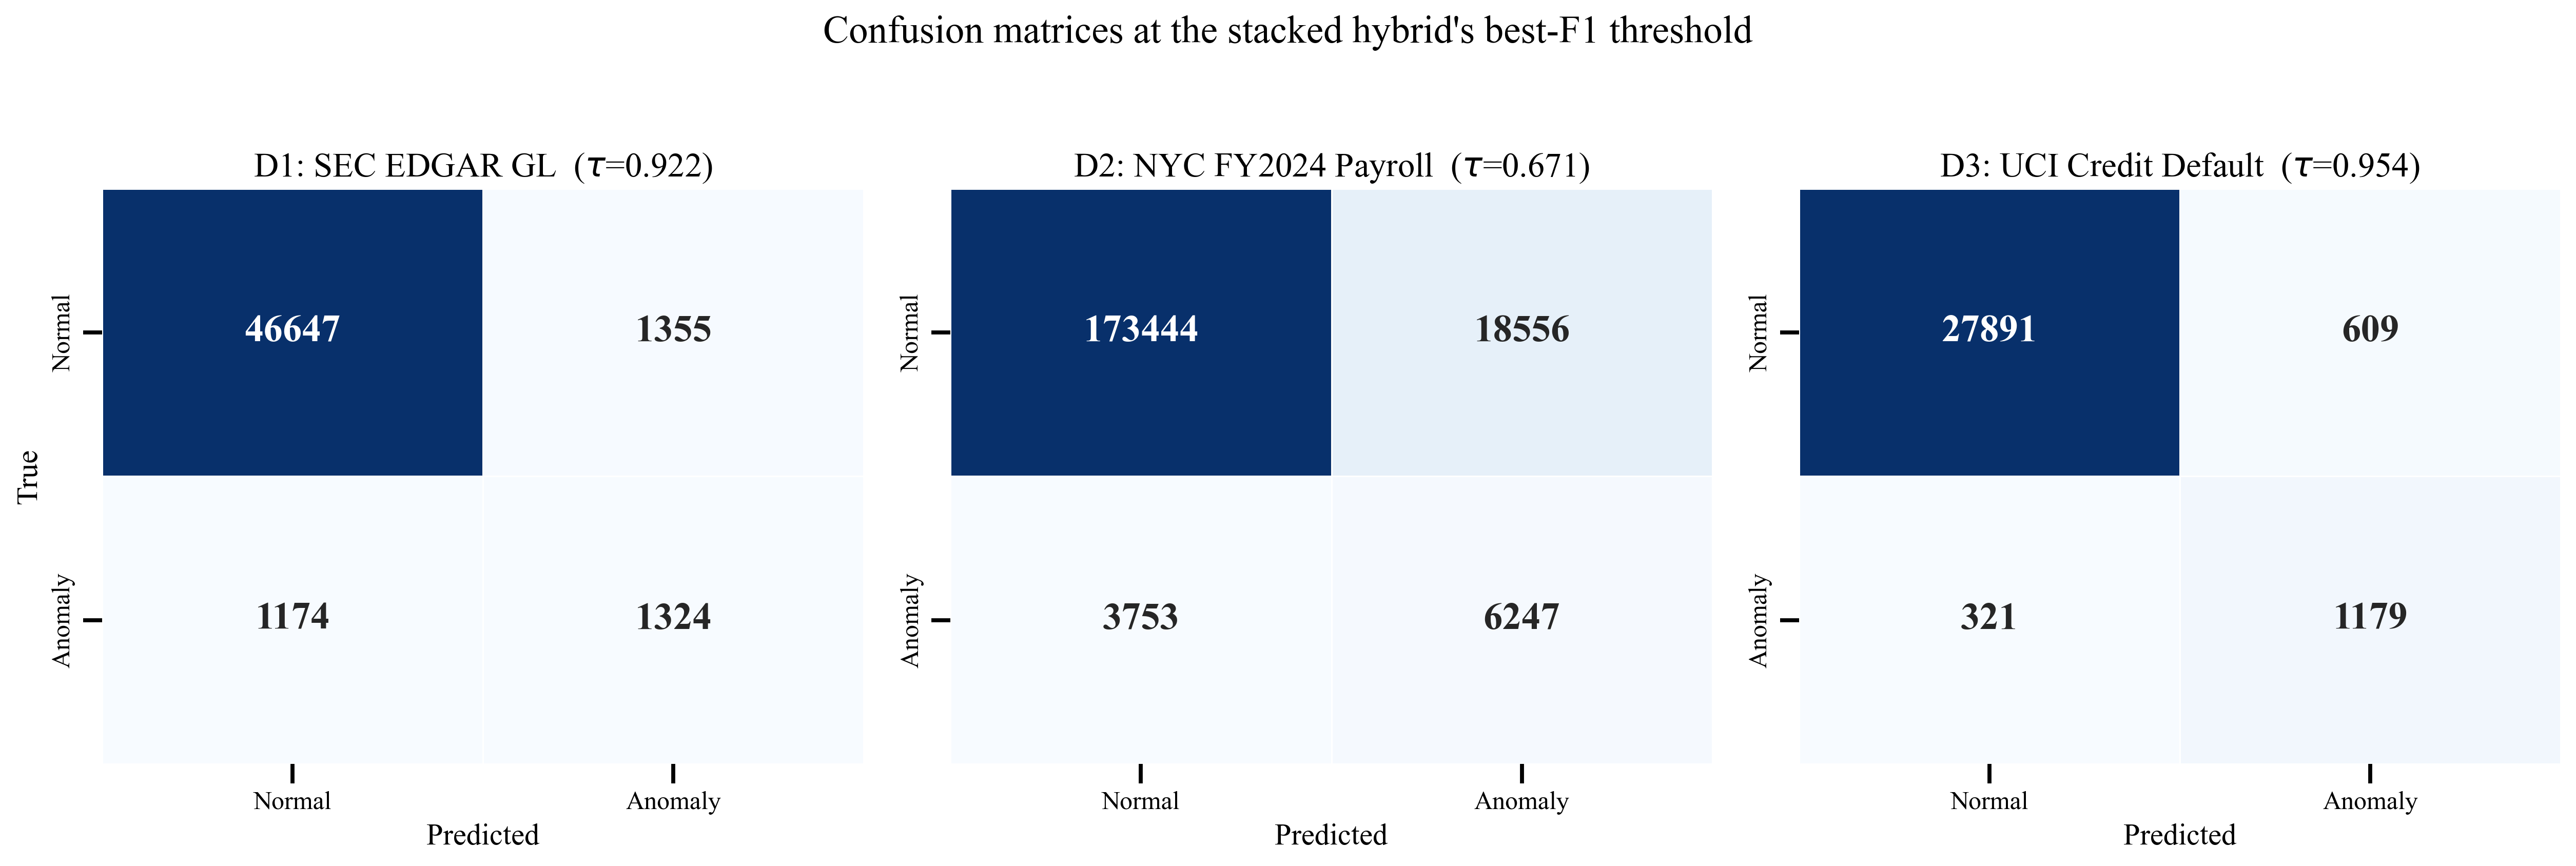
\includegraphics[width=0.9\textwidth]{figures/fig3_confmat.png}
\caption{Confusion matrices at the stacker's best-F1 threshold. False-positive
volume is dominated by D2, which exhibits the largest near-duplicate residual.}
\label{fig:confmat}
\end{figure*}

\subsection{Cross-Validation and Ablation}

Stratified five-fold cross-validation confirms that the point estimates are
stable: F1 standard deviations across folds are 0.010 on D1, 0.004 on D2, and
0.007 on D3 (Table~\ref{tab:cv}). The leave-one-detector-out ablation
(Table~\ref{tab:ablation}, visualised in Fig.~\ref{fig:ablation}) shows that the
most informative single detector varies by dataset---robust statistics on D1
($-0.063$ F1 when removed), the Isolation Forest on D2 ($-0.014$), and the rule
layer on D3 ($-0.027$)---while removing LOF is the least damaging everywhere,
consistent with its weak baseline scores. The variation reinforces the case for
learned rather than fixed fusion.

\begin{table}[tbp]
\centering
\caption{Stratified 5-Fold Cross-Validated Metrics for hybrid$_{\text{LR}}$ (Mean $\pm$ Std)}
\label{tab:cv}
\small
\begin{tabular}{|c|c|c|c|}
\hline
\textbf{Dataset} & \textbf{Precision} & \textbf{Recall} & \textbf{F1} \\
\hline
D1 & $0.500 \pm 0.022$ & $0.513 \pm 0.030$ & $0.506 \pm 0.010$ \\ \hline
D2 & $0.252 \pm 0.003$ & $0.622 \pm 0.008$ & $0.359 \pm 0.004$ \\ \hline
D3 & $0.660 \pm 0.015$ & $0.785 \pm 0.013$ & $0.717 \pm 0.007$ \\ \hline
\end{tabular}
\end{table}

\begin{table}[tbp]
\centering
\caption{Leave-One-Detector-Out From the Stacker. $\Delta$F1 Is Full F1 Minus the Leave-One-Out F1}
\label{tab:ablation}
\small
\begin{tabular}{|l|c|c|c|}
\hline
\textbf{Removed} & \textbf{D1 $\Delta$F1} & \textbf{D2 $\Delta$F1} & \textbf{D3 $\Delta$F1} \\
\hline
rule    & $-0.002$ & $-0.019$ & $+0.027$ \\ \hline
stat    & $+0.063$ & $+0.002$ & $+0.015$ \\ \hline
iforest & $+0.028$ & $+0.014$ & $-0.008$ \\ \hline
lof     & $+0.001$ & $+0.000$ & $+0.011$ \\ \hline
\end{tabular}
\end{table}

\begin{figure}[tbp]
\centering
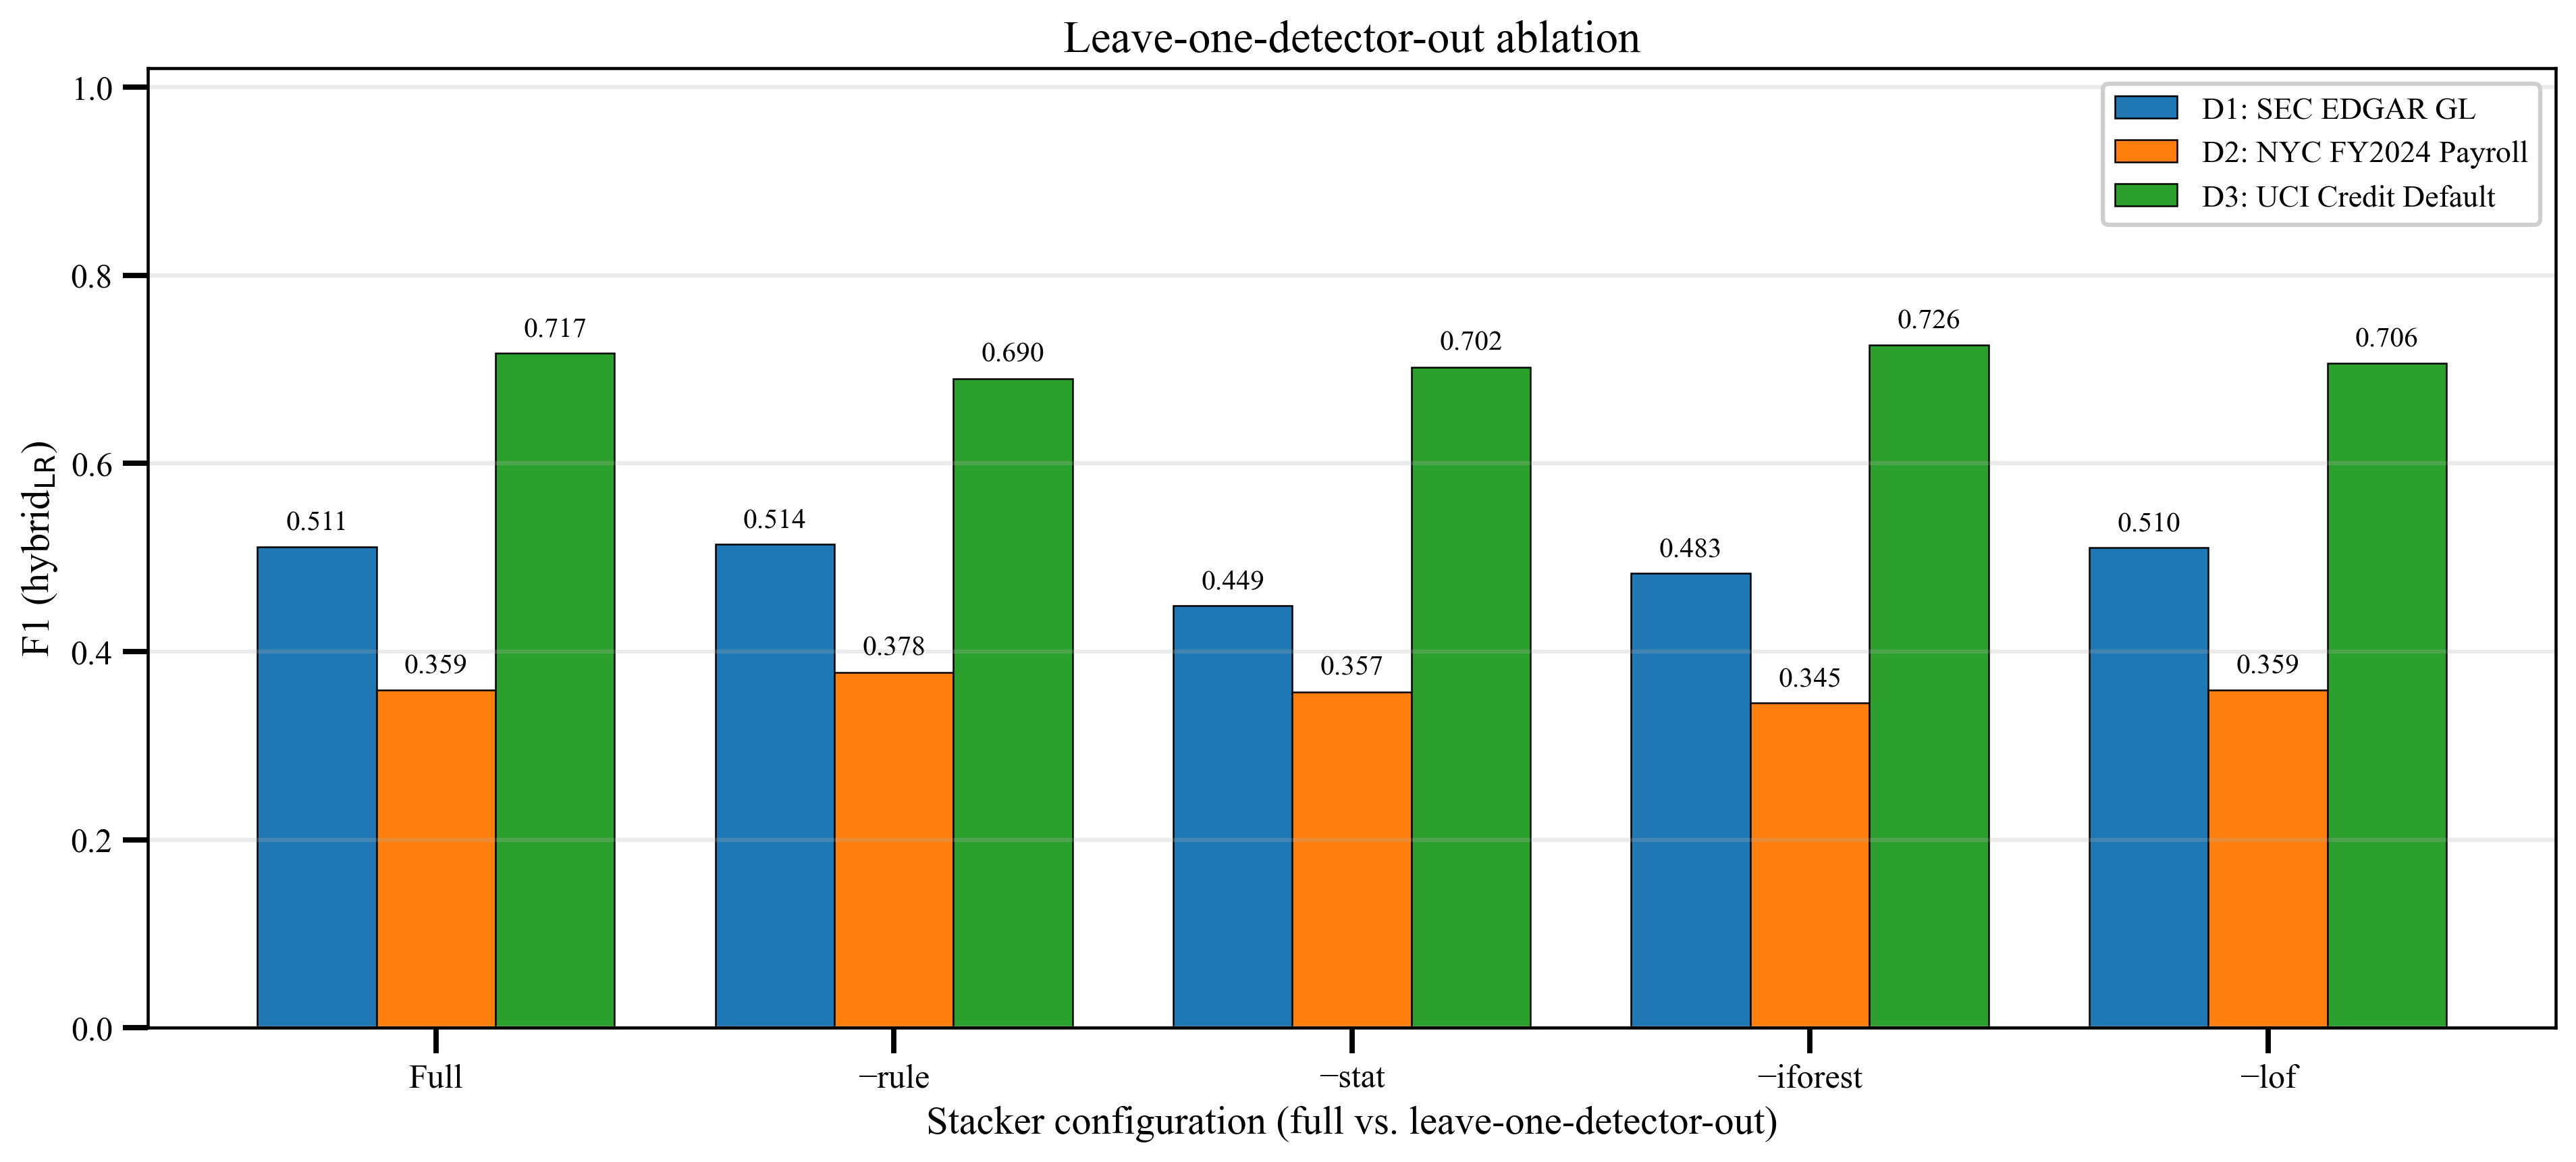
\includegraphics[width=\columnwidth]{figures/fig7_ablation.png}
\caption{F1 after removing each base detector from the stacker (full F1 is the
``none'' bar). The most damaging removal differs by dataset.}
\label{fig:ablation}
\end{figure}

\subsection{Scalability}

We ran the full pipeline on deterministic sub-samples of the payroll corpus at
$n \in \{10\,000, 50\,000, 100\,000, 200\,000\}$. Wall-clock time grows linearly
with $n$, from 0.48 s to 17.32 s (about $87\,\mu$s per row), and F1 is stable
around 0.33--0.35 across sizes (Table~\ref{tab:scalability},
Fig.~\ref{fig:scalability}). The linear profile means the system handles the
largest of the three corpora on a single CPU core without distributed execution.

\begin{table}[tbp]
\centering
\caption{Scalability on D2 Sub-Samples (Single CPU Core)}
\label{tab:scalability}
\small
\begin{tabular}{|r|r|r|c|c|}
\hline
\textbf{$n$} & \textbf{Time (s)} & \textbf{Rows/s} & \textbf{F1} & \textbf{Recall} \\
\hline
10{,}000  & 0.48  & 20{,}659 & 0.350 & 0.568 \\ \hline
50{,}000  & 2.74  & 18{,}279 & 0.334 & 0.624 \\ \hline
100{,}000 & 7.25  & 13{,}785 & 0.348 & 0.619 \\ \hline
200{,}000 & 17.32 & 11{,}545 & 0.331 & 0.613 \\ \hline
\end{tabular}
\end{table}

\begin{figure}[tbp]
\centering
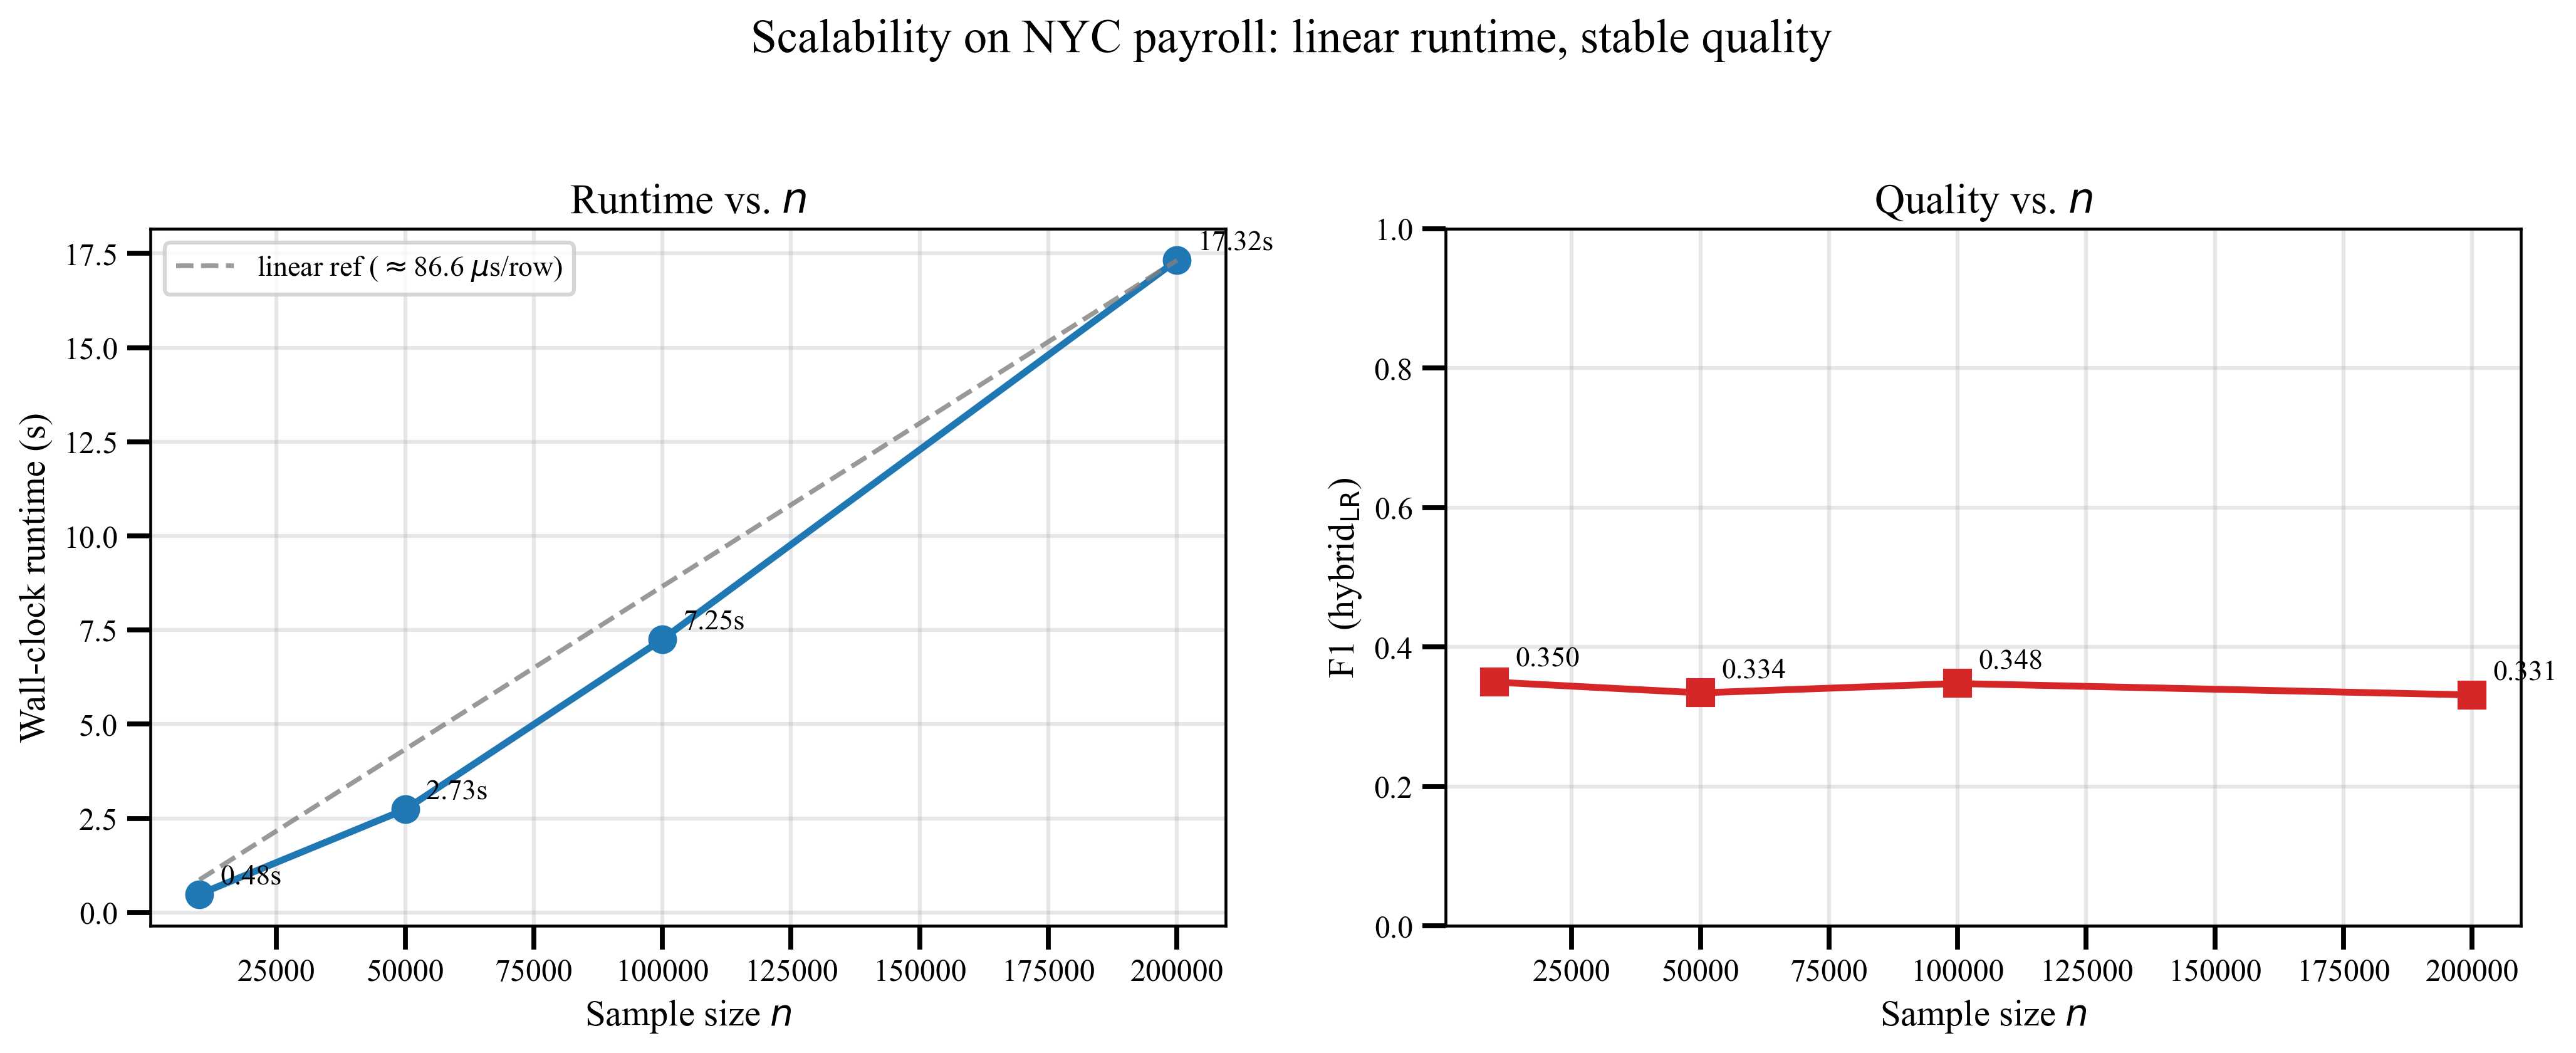
\includegraphics[width=\columnwidth]{figures/fig5_scalability.png}
\caption{Scalability on NYC payroll. Wall-clock time grows linearly with $n$,
while F1 is stable across sizes.}
\label{fig:scalability}
\end{figure}

\subsection{Cross-Dialect SQL Transpilation}

Across the 575 source--target pairs (Table~\ref{tab:sqloverall}), parse and
transpile success are both 0.991, reflecting the maturity of
\texttt{sqlglot}~\cite{mao2024sqlglot} on standard SQL; the only failures are
PostgreSQL queries with \texttt{NULLS LAST} inside window-function frames, Oracle
and Snowflake \texttt{PIVOT}, and Snowflake \texttt{CREATE STREAM}---all
dialect-specific constructs. The substantive number is the strict AST-footprint
equivalence rate of 0.800 overall, which is the share of pairs whose structural
content survives the round trip unmodified.

\begin{table}[tbp]
\centering
\caption{Overall SQL Transpilation Outcomes Across 575 Source--Target Pairs}
\label{tab:sqloverall}
\small
\begin{tabular}{|l|c|}
\hline
\textbf{Metric} & \textbf{Value} \\
\hline
Queries                       & 109 \\ \hline
Source--target pairs          & 575 \\ \hline
Parse rate                    & 0.991 \\ \hline
Transpile rate                & 0.991 \\ \hline
AST-equivalence rate (strict) & \textbf{0.800} \\ \hline
Mean latency (ms)             & 1.09 \\ \hline
P95 latency (ms)              & 2.51 \\ \hline
\end{tabular}
\end{table}

Equivalence varies markedly by dialect pair (Fig.~\ref{fig:sqlmatrix}).
Same-dialect round-trips are at or above 0.92, but several cross-dialect cells
drop below 0.65: Oracle$\rightarrow$MySQL (0.462), Oracle$\rightarrow$T-SQL
(0.538), and Snowflake$\rightarrow$PostgreSQL (0.571). The most common cause is
loss-on-emit of dialect-specific decorators---for example Oracle \texttt{NUMBER}
precision or T-SQL bracket identifiers---that \texttt{sqlglot} legitimately drops
but whose absence changes the AST footprint. Equivalence also degrades with
difficulty (Table~\ref{tab:sqldifficulty}): 0.921 on easy, 0.738 on medium, and
0.742 on hard queries. This is the real, dialect-level signal that
transpile-success alone hides, and it directly answers the surface-metric gap of
Section~\ref{sec:introduction}.

\begin{figure}[tbp]
\centering
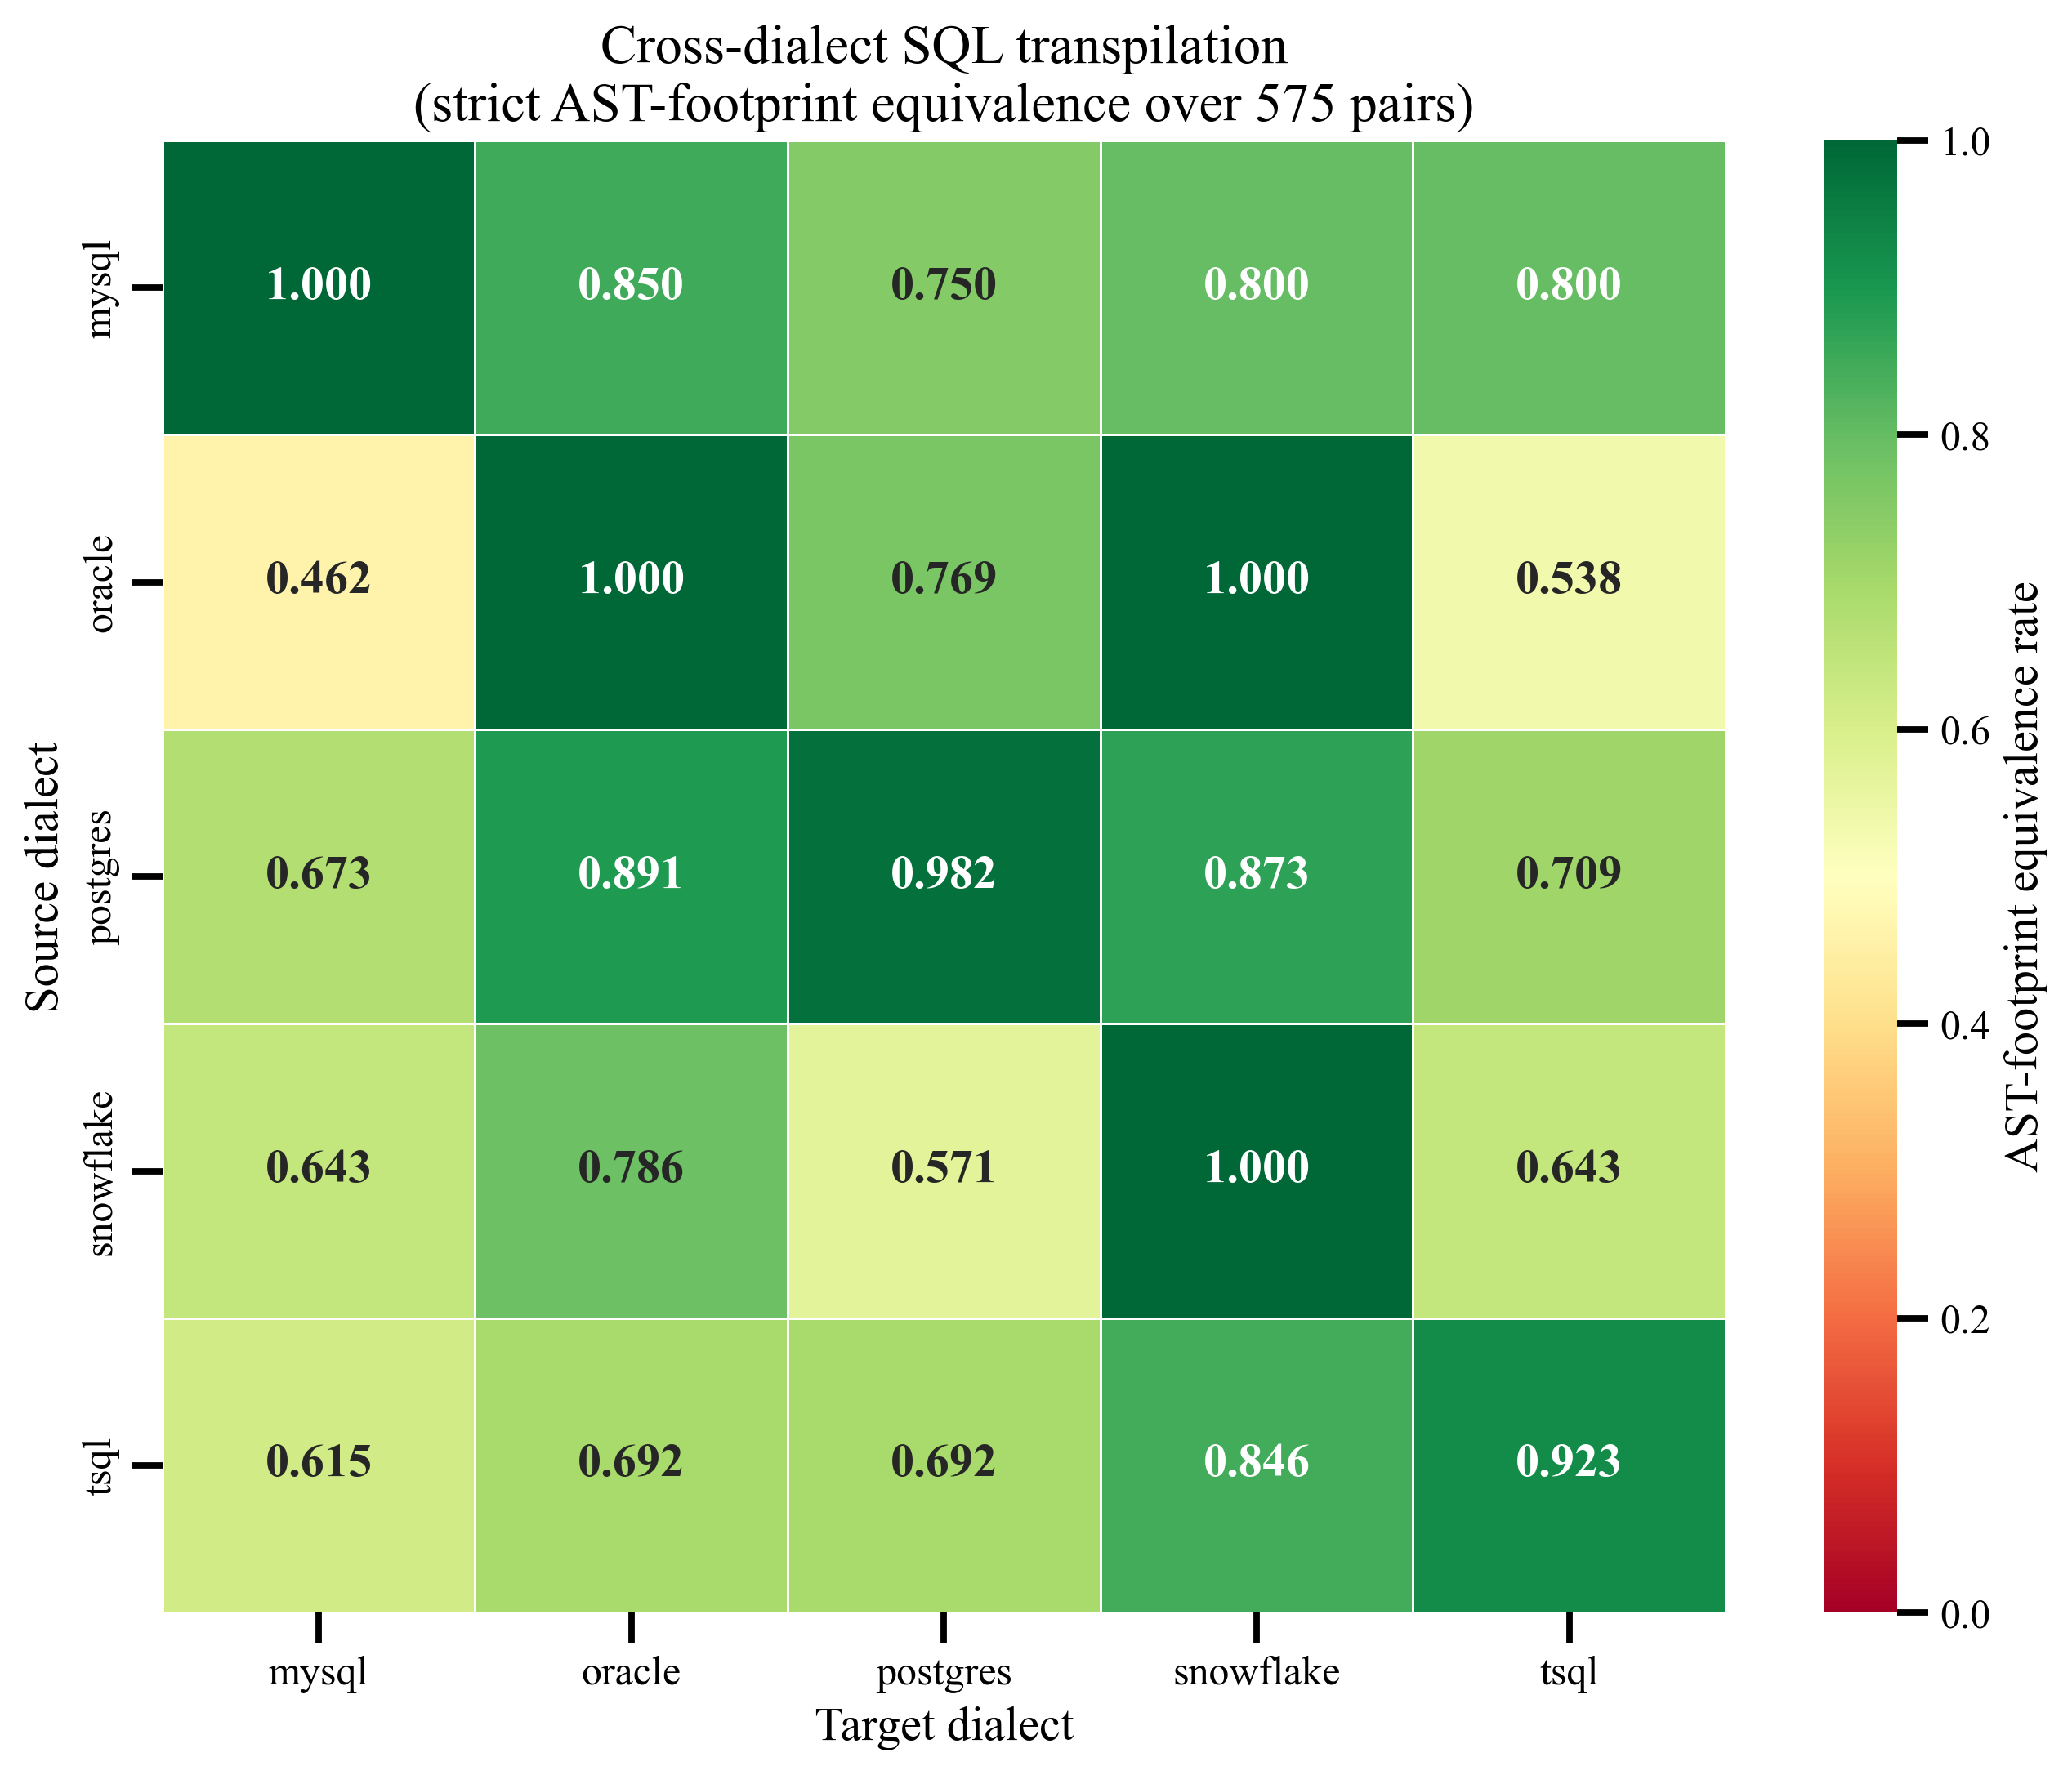
\includegraphics[width=\columnwidth]{figures/fig8_sql_matrix.png}
\caption{AST-footprint equivalence for cross-dialect SQL transpilation. Diagonal
cells are identity round-trips; off-diagonal cells drop where dialect-specific
decorators are lost on emit.}
\label{fig:sqlmatrix}
\end{figure}

\begin{table}[tbp]
\centering
\caption{SQL Transpilation Outcomes Stratified by Query Difficulty}
\label{tab:sqldifficulty}
\small
\begin{tabular}{|l|c|c|c|c|}
\hline
\textbf{Difficulty} & \textbf{$n$} & \textbf{Parse} & \textbf{Transpile} & \textbf{AST-equiv.} \\
\hline
easy   & 190 & 1.000 & 1.000 & 0.921 \\ \hline
medium & 195 & 1.000 & 1.000 & 0.738 \\ \hline
hard   & 190 & 0.974 & 0.974 & 0.742 \\ \hline
\end{tabular}
\end{table}

\subsection{Confidence-Score Geometry}

Operators rarely accept a single threshold without understanding the underlying
score geometry. Fig.~\ref{fig:confdist} plots the stacker output for clean and
injected rows on a log-density scale, with the selected $\tau^{*}$ overlaid.
Three observations follow. D3 is bimodal almost to the point of separability,
which is why its F1 ceiling is the highest of the three corpora. D1 also
separates cleanly at the right tail but carries a heavier mid-range overlap,
reflecting the families (A2, A3) whose discriminative signal is intentionally
absent from the engineered features. D2 is the hardest: the two populations
overlap heavily through the $\hat{s}\in[0.2,0.6]$ band, and any threshold there
trades precision for recall in steep increments. The density view also explains
why $\tau^{*}$ varies so much across datasets---the audit cut sits near the local
minimum between the two modes, which is dataset-specific by construction.

\begin{figure}[tbp]
\centering
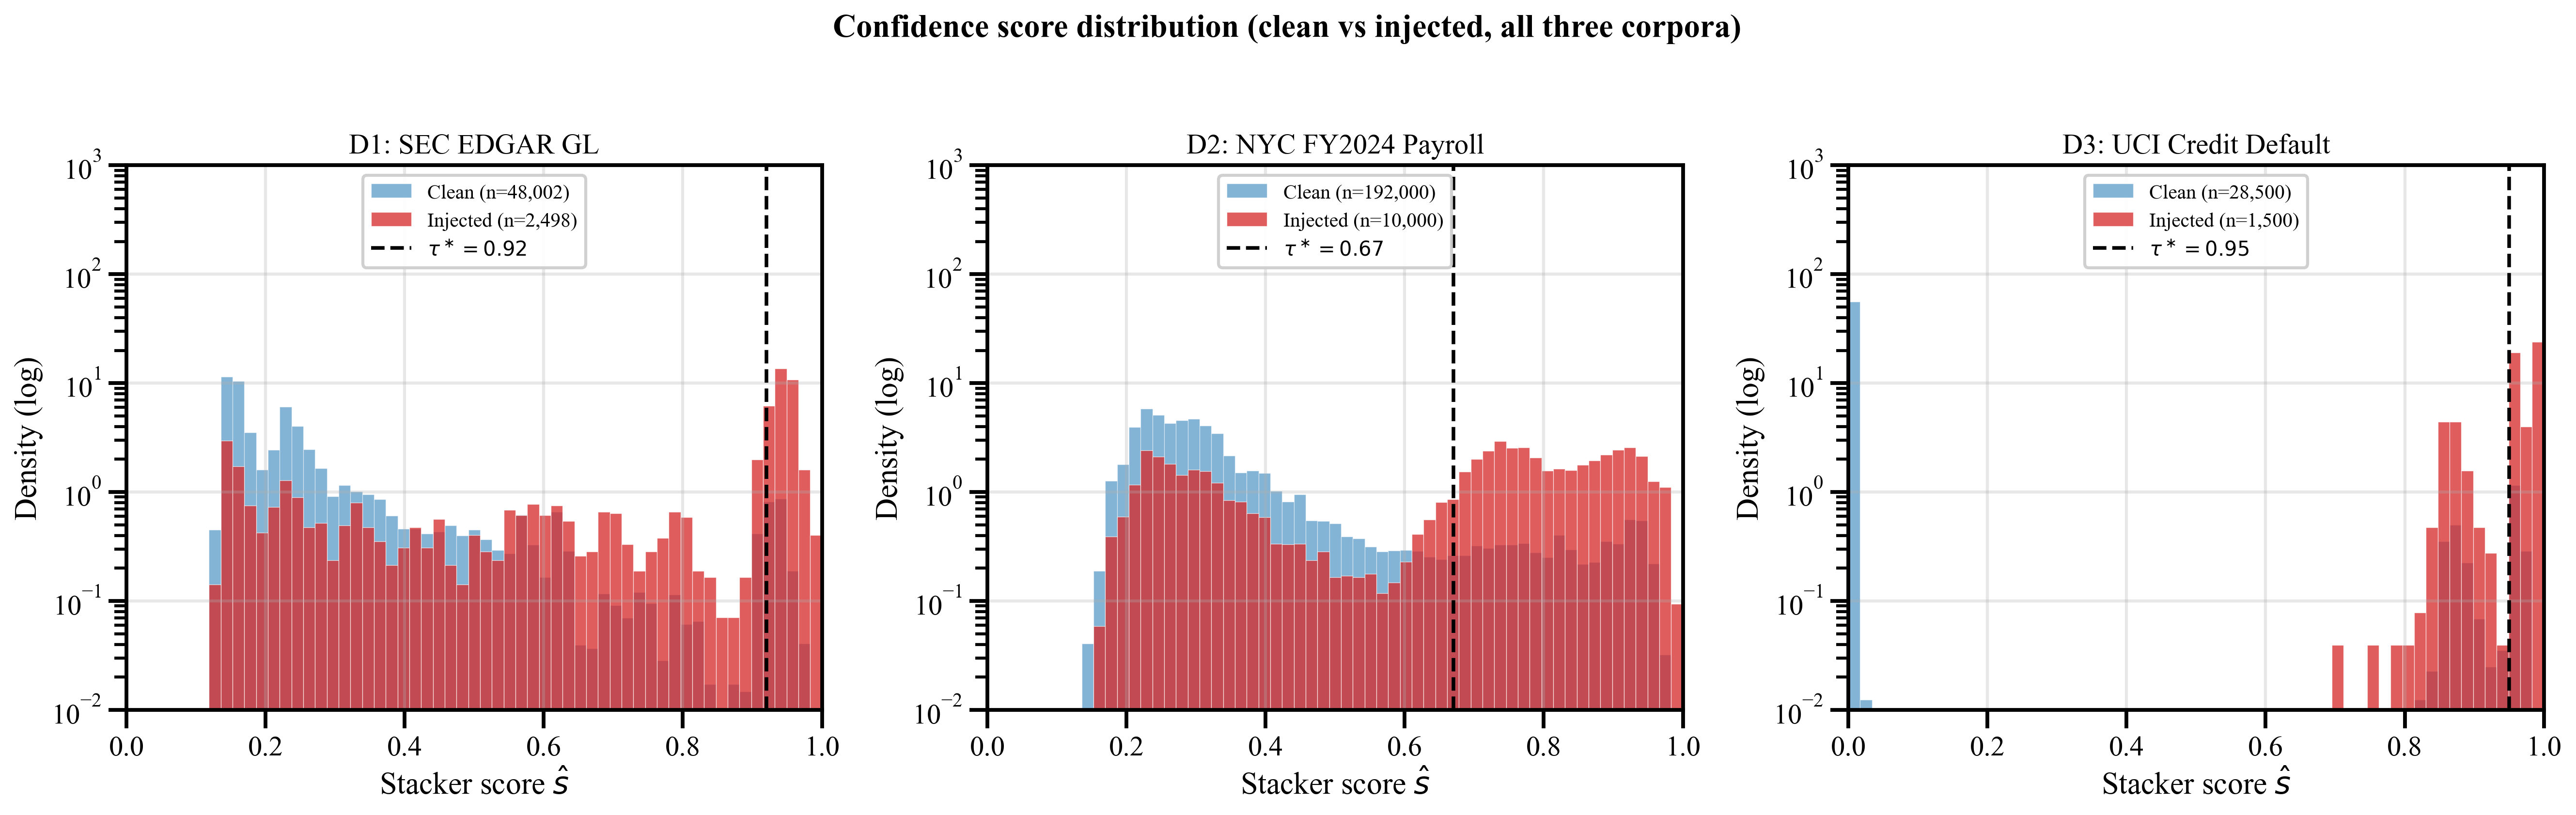
\includegraphics[width=\columnwidth]{figures/fig10_confidence_dist.png}
\caption{Stacker score density on a log scale, separated by ground-truth label.
The dashed line is the dataset-specific $\tau^{*}$ at peak F1. D3 is close to
separable; D2 is not.}
\label{fig:confdist}
\end{figure}

\subsection{Failure Analysis}

We re-examined the 115 source--target pairs where the AST-footprint check rejects
a translation that otherwise parses and transpiles. Hand-classified into five
buckets (Table~\ref{tab:failure}, Fig.~\ref{fig:failure}), the failures are not
uniformly distributed. Decorator and footprint drift account for 62 pairs and is
the dominant mode: \texttt{sqlglot} silently drops dialect hints (Oracle
\texttt{NUMBER(p,s)} precision, T-SQL bracket-quoted identifiers, Snowflake
\texttt{COPY GRANTS}) that have no target equivalent, so the post-transpile AST
carries fewer tokens than the source. These translations execute correctly but
fail strict structural equivalence. Dialect-specific constructs (24 pairs) cover
\texttt{LATERAL}, \texttt{QUALIFY}, \texttt{LISTEN/NOTIFY},
\texttt{generate\_series}, and \texttt{jsonb} operators. Function semantics
(15 pairs) cover \texttt{DATE\_FORMAT}, \texttt{TRY\_CONVERT}, and \texttt{FORMAT},
whose argument order and null behaviour differ across dialects. DML/DDL extensions
(9 pairs) cover \texttt{INSERT IGNORE}, \texttt{CREATE STREAM}, and \texttt{PIVOT}.
Only 5 pairs fail at the parser, all on PostgreSQL queries whose extensions sit
outside the grammar that \texttt{sqlglot} formally supports.

The takeaway for practitioners is operational: the 0.800 AST-equivalence headline
partitions into a large bucket whose ``failures'' are cosmetic decorator drift and
typically harmless at runtime, a smaller bucket of genuinely lossy translations
that require manual review, and a residual of five unparseable inputs that surface
as hard errors at ingestion. An audit pipeline can therefore auto-promote the
cosmetic-drift category while routing only the other two to a human reviewer.

\begin{table}[tbp]
\centering
\caption{Hand-Classified Failure Modes Across the 115 Failing Source--Target Pairs}
\label{tab:failure}
\footnotesize
\setlength{\tabcolsep}{3pt}
\begin{tabularx}{\columnwidth}{|>{\raggedright\arraybackslash}X|c|>{\raggedright\arraybackslash}X|}
\hline
\textbf{Cause} & \textbf{Pairs} & \textbf{Representative Example} \\
\hline
Decorator / footprint drift & 62 & Oracle \texttt{NUMBER(p,s)} $\rightarrow$ MySQL \\ \hline
Dialect-specific construct  & 24 & \texttt{LATERAL} join pg $\rightarrow$ oracle \\ \hline
Function semantics          & 15 & T-SQL \texttt{TRY\_CONVERT} $\rightarrow$ pg \\ \hline
DML / DDL extension         & 9  & MySQL \texttt{INSERT IGNORE} $\rightarrow$ tsql \\ \hline
Parse error                 & 5  & pg \texttt{LISTEN/NOTIFY} \\ \hline
\end{tabularx}
\end{table}

\begin{figure*}[tp]
\centering
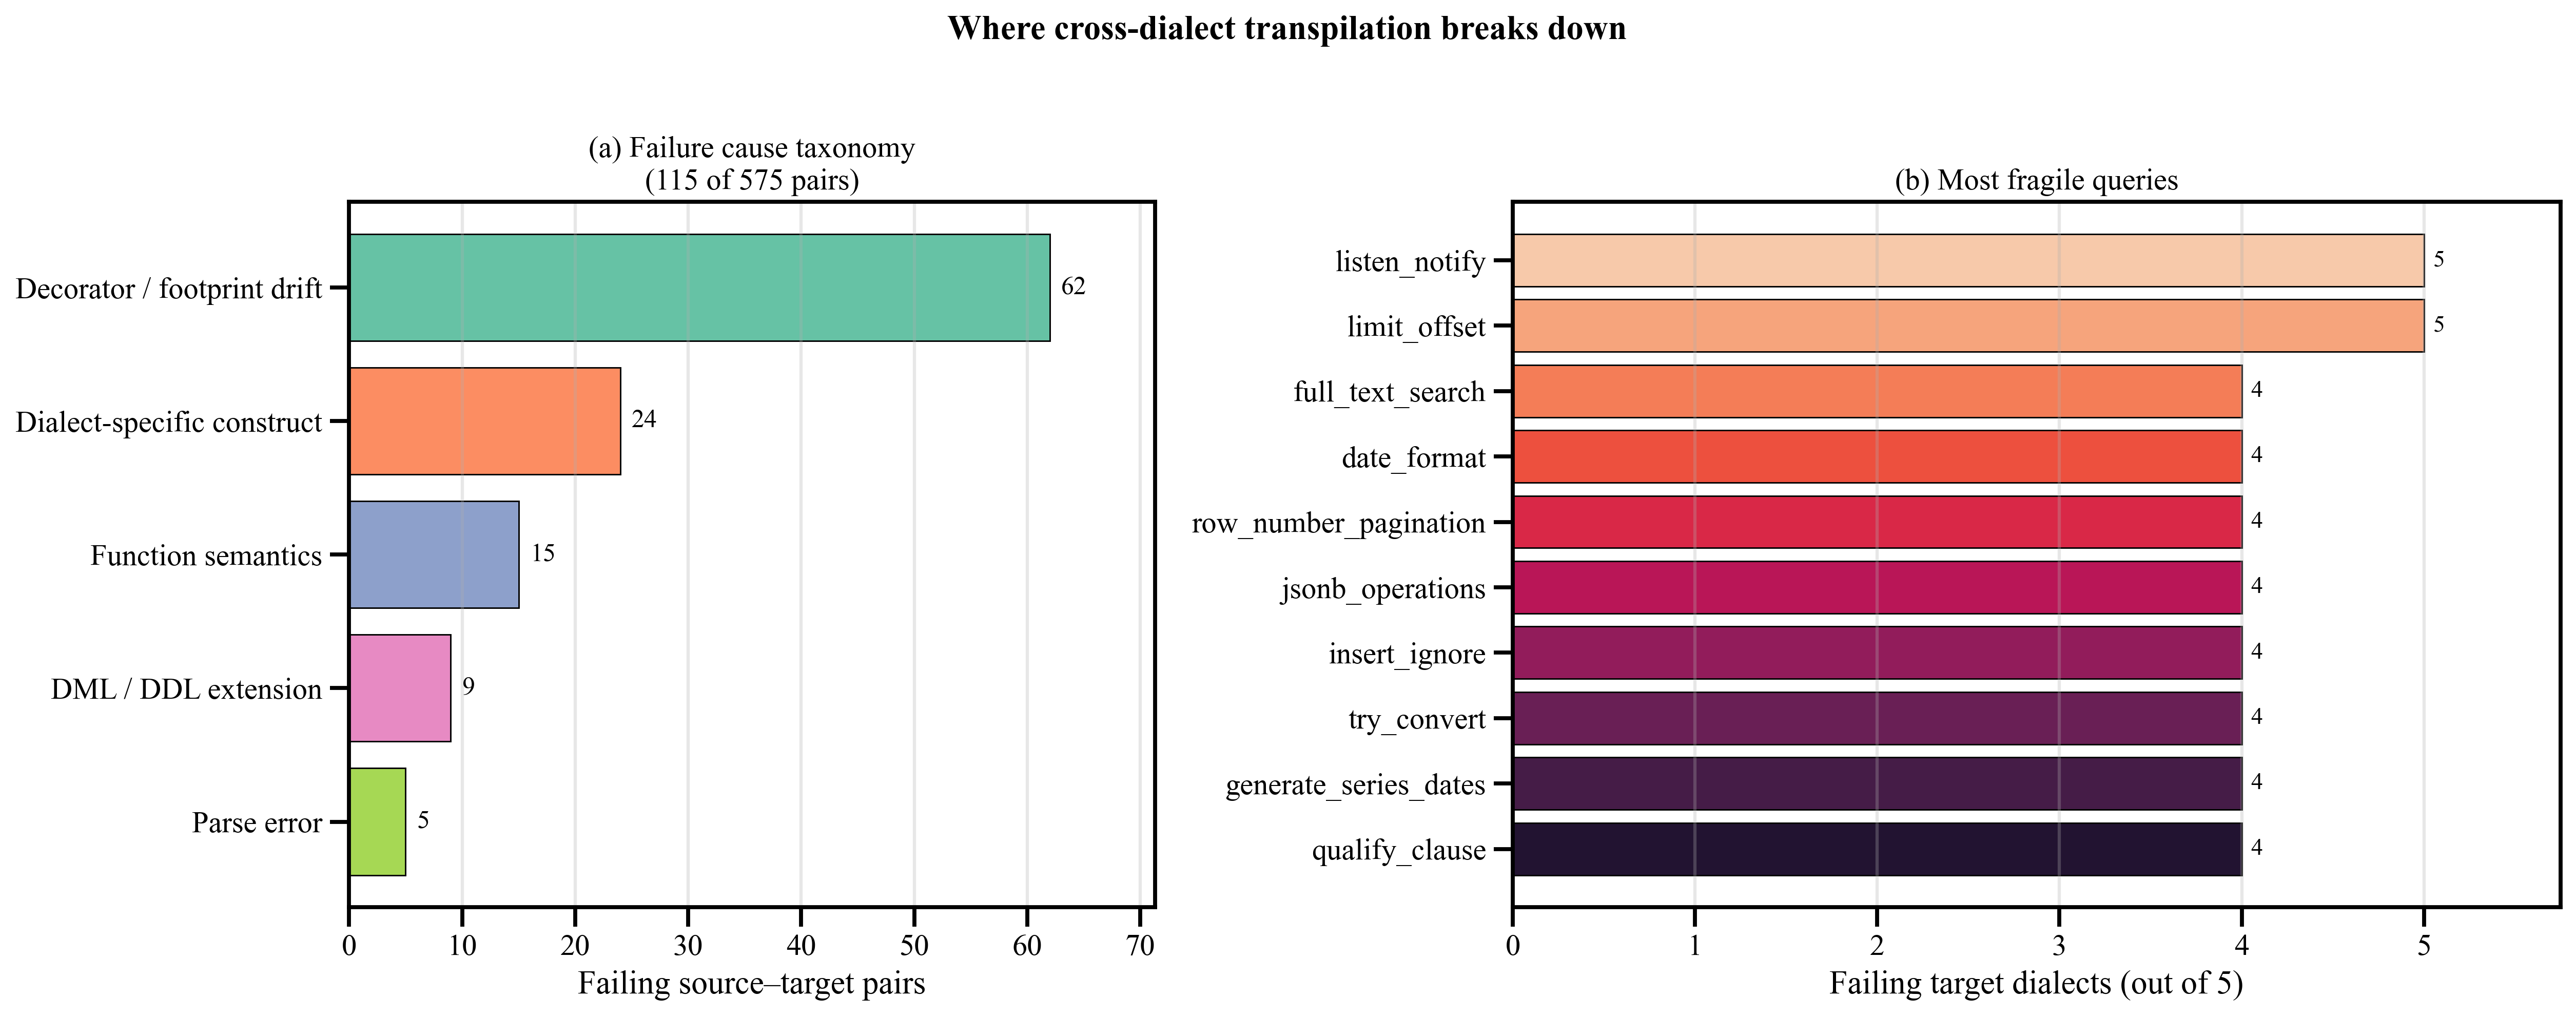
\includegraphics[width=0.9\textwidth]{figures/fig9_failure_analysis.png}
\caption{(a) Cause taxonomy and (b) the ten most fragile queries in the corpus.
The dominant failure mode is loss-on-emit of dialect-specific decorators, not raw
translation errors.}
\label{fig:failure}
\end{figure*}

% =======================================================================
\section{Enterprise Case Study}
\label{sec:casestudy}

To make the end-to-end flow concrete, we trace two real artefacts through the
pipeline: one anomalous record from the SEC corpus and one fragile cross-dialect
query from the SQL corpus (Fig.~\ref{fig:casestudy}).

\begin{figure*}[!tbp]
\centering
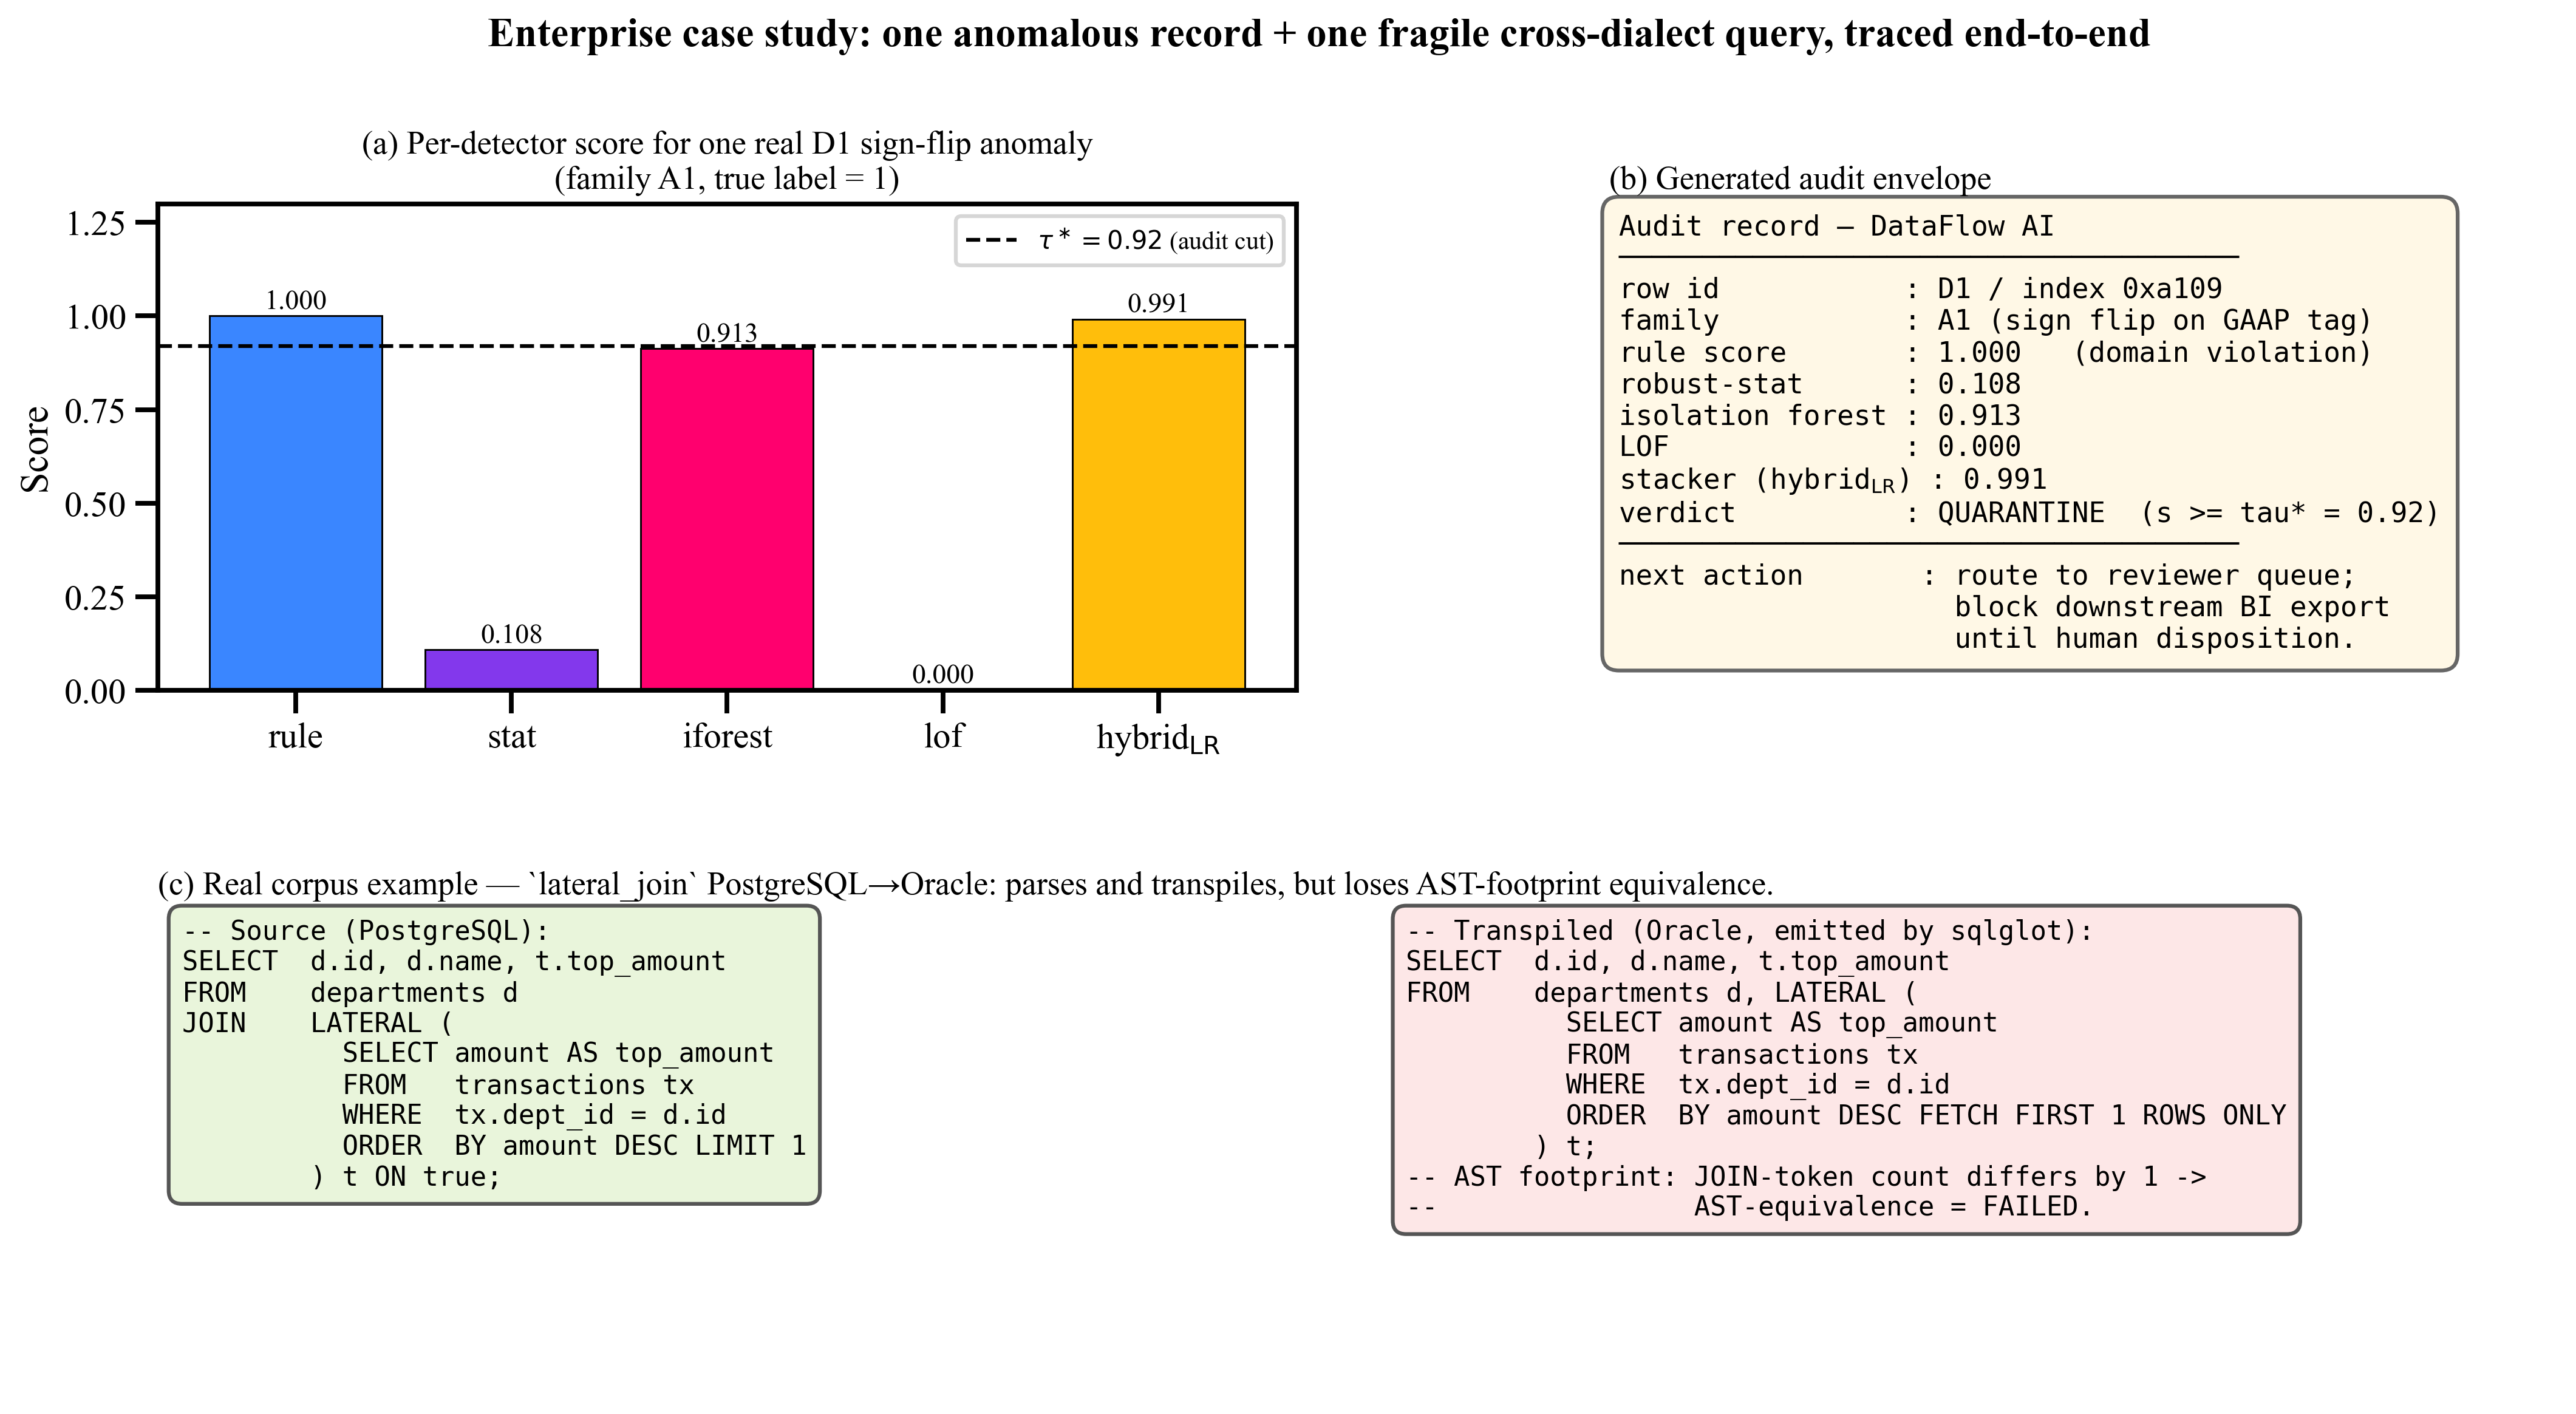
\includegraphics[width=0.95\textwidth]{figures/fig11_case_study.png}
\caption{End-to-end case study. (a) Per-detector scores for one real D1 sign-flip;
the stacker correctly fuses the strong rule/Isolation-Forest signal past the audit
cut. (b) The audit envelope that DataFlow AI emits for downstream review. (c) A
real \texttt{LATERAL}-join PostgreSQL$\rightarrow$Oracle transpile that parses but
loses AST footprint.}
\label{fig:casestudy}
\end{figure*}

\subsection{Anomalous-Record Trace}

The record is index \texttt{0xa109} of D1, an injected A1 sign-flip on a U.S. GAAP
tag constrained to be non-negative. The rule layer returns 1.000 because the
domain check fires deterministically. The Isolation Forest agrees (0.913) because
the negated value lies in the extreme left tail of the per-tag distribution. The
robust-stat detector returns only 0.108: the magnitude is plausible for the
surrounding tags, so the per-group $z$-score is small---exactly the kind of
correlated-but-weak signal that motivates a learned stacker rather than a fixed
average. LOF returns 0.000 because the record's neighbours in the engineered
feature space are also altered by the same family. The logistic-regression stacker
fuses these into 0.991, which exceeds the D1 audit cut $\tau^{*}=0.92$ and routes
the record to the quarantine sink with a structured audit envelope.

\subsection{Migration Trace}

The query is a \texttt{LATERAL} join from the PostgreSQL corpus, transpiled to
Oracle. Both stages succeed: the parser accepts the PostgreSQL form, and
\texttt{sqlglot} emits a syntactically valid Oracle query that an Oracle planner
will execute. The AST-footprint test, however, rejects the pair: the PostgreSQL
\texttt{JOIN LATERAL ... ON true} compiles into a single \texttt{JOIN} AST node,
while the Oracle output renders the lateral as a comma-separated \texttt{FROM}
reference that the Oracle parser materialises as zero \texttt{JOIN} nodes. The
token count differs by one, so the structural-equivalence check returns false.
This is a decorator-drift failure in the taxonomy of the previous section: the
executed semantics are identical, but the AST footprint changes. A production
audit gate that wants to keep this query in the auto-promote lane needs either a
normalised lateral-rewriting rule or a relaxed footprint comparator that treats
\texttt{JOIN} and comma-list \texttt{FROM} clauses as the same node class.

% =======================================================================
\section{Discussion}
\label{sec:discussion}

\subsection{When Does the Stacker Actually Help?}

The stacker dominates the fixed-weight hybrid where the base detectors disagree
informatively---on the SEC filings, where rule-based GAAP constraints carry most
of the signal, and on UCI credit default, where four of five injected families
admit rule-level discrimination. On payroll, the base detectors are highly
correlated and the stacker's gain over the fixed-weight hybrid is statistically
negligible, yet it still trades roughly 0.105 of additional recall for a
controlled FPR uplift, which is the relevant operating regime for audit
applications. The practical lesson is that learned fusion is most valuable
precisely where a single hand-set weight vector would mis-rank the
detectors---and that the threshold sweep, not the point estimate, is what lets an
operator choose the operating point that matches the cost asymmetry of the task.

\subsection{Coupling Integrity and Migration in One Gate}

The case study is deliberately small, but it illustrates the operational point
behind the unified design. The anomalous record becomes a real risk only once it
survives ingestion; the fragile query becomes a real risk only once it is shipped
against the underlying tables. Decoupling the two checks lets each pass on its own
narrow criterion---``the row looks fine to the detector'' and ``the SQL still
compiles''---while the joint failure mode, a wrong number computed by a
correct-looking query over a corrupted row, slips through. Wiring both into a
single audit envelope gives downstream reviewers one artefact to act on, which is
the property that justified the additional engineering of the unified contract.

\subsection{The Transpile-Success Tripwire}

A pre-registered tripwire halts and reports any metric exceeding 0.99. Parse and
transpile rates both fired at 0.9913. We report this transparently rather than
masking it: \texttt{sqlglot} is a mature parser, and on a corpus that is largely
standard ANSI/ISO SQL plus well-supported extensions, parse and transpile success
should approach the ceiling. The strict AST-equivalence rate of 0.800 is the
metric we recommend for evaluation going forward; it does not trip the wire and it
exposes the dialect-pair gradient that parse-success obscures. This is a concrete
instance of the trustworthy-AI principle that production metrics must measure what
matters operationally rather than what is easiest to
saturate~\cite{kaur2023trustworthy, li2023trustworthy}.

\subsection{Threats to Validity}

\textbf{Anomaly injection.} Although every family is grounded in documented audit
failure modes, injected anomalies are not field-discovered errors. We mitigate
this by reporting per-family recall so that practitioners can re-weight families
to their domain, and by holding prevalence near a realistic five percent rather
than the inflated rates common in synthetic studies.
\textbf{Dataset selection.} Three datasets cannot represent every enterprise
context; we chose them for domain diversity---regulated reporting, public-sector
compensation, and consumer credit---and for licence clarity.
\textbf{SQL corpus.} The 109-query corpus is curated rather than random, so
dialect-specific failure modes are over-represented; the equivalence matrix should
be read as a worst case rather than an expected production rate.
\textbf{Hardware.} All timings are single-CPU; the linear scaling we observe is
plausible to improve with parallel trees, but multi-core behaviour is not measured
here.

% =======================================================================
\section{Conclusion and Future Work}
\label{sec:conclusion}

We presented DataFlow AI, a deployment-oriented framework that couples a stacked
anomaly-detection ensemble with an AST-verified cross-dialect SQL transpiler under
a single reproducibility contract. On three real public corpora---SEC EDGAR, NYC
payroll, and UCI credit default---the logistic-regression stacker improves over
the strongest single detector on two of three datasets (F1 of 0.511 and 0.717 on
D1 and D3) and matches it on the third while shifting the precision/recall
trade-off in favour of recall, with per-family reporting that names exactly which
anomaly types the system catches and which it misses. On 575 cross-dialect SQL
pairs the strict AST-equivalence rate is 0.800 overall and varies predictably with
query difficulty and dialect pair, exposing where transpile-success metrics are
optimistic; a failure-mode taxonomy further partitions that headline into a large
cosmetic-drift bucket an audit pipeline can safely auto-promote and a smaller
bucket of genuinely lossy translations that must be reviewed by hand. The
contribution is therefore not a new accuracy record but a transparent,
reproducible demonstration that deployment-aware, confidence-coupled integration
of validation and migration is both feasible and operationally sensible---subject
to the clearly stated limits of injected evaluation, which expert-annotated and
real-world studies should next address. All code, anomaly masks, and
SHA-256-verified datasets reproduce end-to-end from a fixed seed.

The limitations follow directly from the threats above. The three anomaly families
with near-zero recall (A2, A3, C3) are limited by feature coverage rather than by
the fusion mechanism, and call for richer learnt features---tag-embedding
similarity for tag-semantics families and signed bill ratios for sign-violation
families. The AST-footprint comparator is intentionally strict and would benefit
from a relaxed mode that treats semantically equivalent renderings (such as
lateral joins and comma-list \texttt{FROM} clauses) as the same node class. More
broadly, the synthetic injection should be complemented by expert-annotated,
field-discovered errors, and the SQL pipeline should be coupled to schema-level
metadata so that AST equivalence can be augmented with execution-time
row-equivalence checks against representative seed data. Near-term work targets
calibration-aware threshold selection~\cite{guo2017calibration,guo2021reliability}
and richer features for the underperforming families; longer-term work targets
multi-domain validation beyond the three corpora studied here.

\EOD

% =======================================================================
\bibliographystyle{IEEEtran}
\bibliography{FINAL_BIBLIOGRAPHY}

% =======================================================================
% Author biographies
% =======================================================================
\vfilneg

\begin{IEEEbiography}[{
\includegraphics[width=1in,height=1.25in,clip,keepaspectratio]{figures/author_upasana.png}}]{UPASANA BHAUMIK}
is an undergraduate student in Computer Science and Engineering with a
specialization in Bioinformatics at Vellore Institute of Technology, India. She
actively builds AI-driven and data-centric applications, combining machine
learning, data engineering, and full-stack development to solve real-world
problems. Her work includes developing intelligent systems for data analysis,
predictive modeling, and interactive applications powered by large language
models. She is particularly interested in leveraging AI for bioinformatics and
healthcare, along with advancing data quality and automation in large-scale
systems.
\end{IEEEbiography}

\vfilneg

\begin{IEEEbiography}[{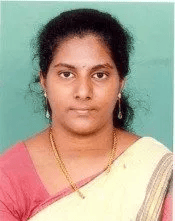
\includegraphics[width=1in,height=1.25in,clip,keepaspectratio]{figures/author_berlin.png}}]{BERLIN M A}
received the master's degree in computer science engineering from National
Engineering College, Tamil Nadu, and the Ph.D. degree in computer science
engineering from Anna University, Chennai. Currently, she is an Associate
Professor with the School of Computer Science and Engineering, Vellore Institute
of Technology, Vellore. Her research interests include ad hoc networks, IoT and
machine learning. She has over 20 years of experience in teaching and research.
She has published many papers in international journals and conferences on
vehicular ad hoc networks, machine learning and deep learning. She has published
few patents on IoT and artificial intelligence.
\end{IEEEbiography}

\end{document}